\documentclass[futureinternet,article,submit,moreauthors]{Definitions/mdpi}

\firstpage{1}
\makeatletter
\setcounter{page}{\@firstpage}
\makeatother
\pubvolume{1}
\issuenum{1}
\articlenumber{0}
\pubyear{2026}
\copyrightyear{2026}
\externaleditor{}
\datereceived{ }
\daterevised{ }
\dateaccepted{ }
\datepublished{ }
\hreflink{https://doi.org/}

\usepackage[utf8]{inputenc}
\usepackage{graphicx}
\usepackage{float}
\usepackage{tabularx}
\usepackage{changepage}
\usepackage{array}
\usepackage{ragged2e}
\usepackage[T1]{fontenc}
\usepackage{booktabs}

% Supervisor feedback: no real DOI has been assigned yet. The MDPI class
% prints the DOI in the regular footer and also in the first-page `plain`
% page style, so blank both here rather than editing the vendor class file.
\rfoot{}
\makeatletter
\fancypagestyle{plain}{%
\renewcommand{\footrulewidth}{0.4pt}
\fancyhead{\null\vspace{8pt}}
\fancyfoot[L]{%
\fontsize{8}{8}\selectfont
\ifthenelse{\equal{\@status}{submit}}{%
Version {\@ \today} submitted to {\em \journalname}%
}{%
{\em\journalname\ }{\bfseries\@pubyear}, {\em \@pubvolume}, %
\ifthenelse{\equal{\@continuouspages}{\@empty}}{%
\@articlenumber %
}{%
\@firstpage\ifnumcomp{\getpagerefnumber{LastPage}}{=}{\@firstpage}{}{--\pageref*{LastPage}} %
}%
}%
}
\fancyfoot[R]{}
}
\makeatother

%=================================================================
\Title{Hybrid Content- and Session-Based Anomaly Detection for Web Server Logs}

% AUTHOR BLOCK. Matches the peer paper's author-role pattern (student
% first/corresponding author, supervisor + moderator as co-authors).
% Moderator's surname confirmed directly by Mr Hassanu as "Hassanu",
% resolving the earlier inconsistency against "Muhsin Hussenu" (thesis
% body/acknowledgements) and "Muhsin Husseinu" (thesis title page).
% ORCID: MDPI requires an ORCID iD for at least the corresponding author.
% Define each author's ORCID below (letters A, B, C map 1:1 to author order),
% then append the matching \orcidX{} icon-link straight after that author's
% name in \Author{} below (e.g. "Abdul Rehman \orcidA{}"). Replace the
% dummy digits with the real ORCID iDs before submission.
% \newcommand{\orcidauthorA}{0000-0000-0000-0000}
% \newcommand{\orcidauthorB}{0000-0000-0000-0000}
% \newcommand{\orcidauthorC}{0000-0000-0000-0000}

\Author{Abdul Rehman *, Mouhammad Nouman and Muhsin Hassanu *}

\AuthorNames{Abdul Rehman, Mouhammad Nouman, and Muhsin Hassanu}

\address[1]{Department of Computing and Cybersecurity, University of the West of Scotland, London Campus, London E14 2BA, UK}

\corres{Correspondence: b01753459@studentmail.uws.ac.uk (A.R.); muhsin.hassanu@uws.ac.uk (M.H.)}

\abstract{Rule-based inspection of web server logs cannot detect attacks it has not already been told to look for, and most anomaly-detection studies validate their methods on a single dataset, which risks overstating how well a method generalises to new traffic. This paper presents a hybrid framework that fuses a content-based autoencoder, which scores individual HTTP requests, with a session-based variational LSTM autoencoder, which scores per-client request sequences. The framework is evaluated across eight datasets spanning three log formats, including the public CSIC~2010 HTTP dataset, under both within-dataset and cross-dataset threshold-transfer protocols. Correcting a session-construction fault that had mixed different clients' requests into the same window raises the session branch's AUC on CSIC~2010 from 0.63 to 0.98, evaluated on a held-out split disjoint from the requests the corrected model was trained on; the branch depends on genuine multi-request sessions and produces no score where the traffic does not contain them. Fusion is not uniformly beneficial: on CSIC~2010, weighting fully toward the session branch outperforms every blended weight tested. A threshold calibrated once on normal CSIC~2010 traffic and transferred unchanged to three attack-heavy datasets raises fused F1 six- to seven-fold over a threshold tuned separately on each dataset, because those datasets contain too much attack traffic for self-calibration to represent normal behaviour. The framework also achieves a lower false positive rate than a labelled Random Forest baseline, at comparable or better AUC than unsupervised baselines, and runs fast enough for near-real-time use. Taken together, these results show that session structure and threshold calibration can matter as much as model choice.}

\keyword{web server logs; anomaly detection; autoencoder; variational LSTM; session modelling; score fusion; cross-dataset evaluation; threshold transfer}

\begin{document}

\section{Introduction} \label{sec1}

Web applications underpin most critical digital services in use today, from banking and healthcare to e-commerce and cloud infrastructure, and their continuous, public-facing exposure makes them a persistent target for attackers~\cite{scarfone2007}. Every request a web server processes is recorded in an access log, together with metadata such as the request method, path, response status, and client identifiers. These logs are one of the richest available sources of security-relevant information: in principle, they capture both the legitimate use of an application and the traces left by attackers probing or exploiting it. In practice, however, the volume and variety of this data make manual inspection infeasible for any application of meaningful scale, and organisations have long relied on signature-based intrusion detection and rule-based filtering to triage it~\cite{scarfone2007}.

Signature- and rule-based approaches are effective against known attack patterns but are structurally unable to detect zero-day or previously unseen attacks, since they can only recognise what has already been catalogued. This has motivated a shift towards anomaly detection, which instead models what \emph{normal} traffic looks like and flags deviations from it, without requiring the deviation to match a predefined signature~\cite{chandola2009}. Anomaly detection is a natural fit for web security because it does not depend on a labelled corpus of known attacks -- which is difficult to obtain, quickly goes stale, and can never be assumed complete -- but it introduces its own difficulties. Web traffic is highly non-stationary: normal behaviour drifts as applications change, and it can vary enormously between different endpoints, user populations, and even times of day. Attack traffic is also typically a tiny fraction of the total volume, so any evaluation of an anomaly detector must be designed around severe class imbalance rather than raw accuracy~\cite{chandola2009}.

Deep learning has extended anomaly detection to log and web-traffic data by learning representations directly from raw or lightly processed records, rather than requiring hand-engineered features. Sequence models such as LSTMs~\cite{hochreiter1997} have been used to learn the normal structure of a stream of log events and flag deviations from it~\cite{nedelkoski2020}, and DeepLog demonstrated that treating a system log as a natural-language-like sequence allows an LSTM to learn normal execution patterns and detect anomalies as departures from them~\cite{du2017}. Applied to HTTP traffic specifically, this behavioural, sequence-oriented view is complementary to a second, request-level view: individual HTTP requests can themselves be modelled directly, using an autoencoder trained to reconstruct the structural and payload characteristics of normal requests, so that unusually large reconstruction error flags anomalous content such as injection payloads or malformed parameters. Recent work combining a variational LSTM autoencoder~\cite{kingma2014,ancho2015} with a deviation network for exactly this purpose has shown that this class of model is well suited to detecting web attacks directly from HTTP weblogs~\cite{jagat2024}.

These two views, however, are not interchangeable. A content-based model that scores individual requests in isolation cannot see attacks that only become apparent across a sequence of otherwise unremarkable requests -- reconnaissance-style scanning, credential stuffing, or low-and-slow probing, for example, where each individual request may be syntactically valid. A behaviour-based model that scores sequences of requests grouped by client can catch exactly this class of attack, but it depends on there being a genuine sequence to model in the first place: if a client only issues one or two requests, or if requests from a given client cannot be reliably grouped together, there is no behavioural signal to learn from. This dependency on session structure is not merely a theoretical caveat -- as this study's own experiments later show (Section~\ref{sec5}), it materially determines whether a session-based branch can contribute anything at all for a given traffic sample.

Because content-based and behaviour-based detectors fail in different, largely non-overlapping ways, combining their outputs is a natural way to cover more of the attack surface than either can alone. Hybrid, fusion-based frameworks that integrate multiple detection signals have been shown to improve robustness and stability relative to single-model detectors, particularly under the kind of severe class imbalance and limited labelled data that characterises real security settings~\cite{kamal2025}. Realising this benefit in practice, however, depends heavily on how the resulting system is evaluated. A large share of the anomaly-detection literature reports results on a single dataset, which risks overstating how well a method will generalise once deployed against traffic with different structure, format, or attack composition than whatever it was tuned against. This concern is well established in the wider intrusion-detection literature, where the design of benchmark datasets themselves -- their realism, diversity, and reproducibility -- has long been recognised as a determining factor in whether reported results are meaningful outside the dataset they were produced on~\cite{shiravi2012}.

Despite the individual maturity of content-based autoencoders, behaviour-based sequence models, and fusion-based detection frameworks, their combined application to web server logs specifically, evaluated across genuinely different log formats and under a strict cross-dataset protocol -- where a detection threshold is fixed on one data source and applied unchanged to others, rather than recalibrated on each dataset in turn -- remains underexplored. Many studies that do combine content and behavioural signals validate the result on a single log format and a single traffic sample, leaving open how such a system behaves when the underlying session structure, log schema, or class balance of the target traffic differs substantially from what the model was built on.

To address this gap, this work presents a hybrid anomaly detection framework for web server logs that combines a content-based autoencoder, trained to reconstruct the structural features of individual HTTP requests, with a session-based variational LSTM autoencoder, trained on genuine per-client request sequences rather than an arbitrary sliding window over the raw log stream. The outputs of the two branches are combined through score-level fusion, and the resulting framework is evaluated not only within a single dataset but across three structurally different sources: two self-generated Apache-style access-log corpora and a structured Nginx JSON log, together with the publicly available CSIC~2010 HTTP dataset, which additionally serves as the source domain for a cross-dataset threshold-transfer evaluation in which a single fixed decision threshold, calibrated once on genuinely benign traffic, is applied unchanged to unseen target datasets.

The remainder of this paper is organised as follows. Section~\ref{sec2} sets out the specific contributions of this work. Section~\ref{sec3} reviews related work on anomaly detection for web and log data, content- and behaviour-based deep learning models, and hybrid/fusion-based detection frameworks. Section~\ref{sec4} describes the datasets, preprocessing, feature representation, model architectures, and evaluation protocol. Section~\ref{sec5} presents the experimental results, including the branch ablation, fusion-weight sensitivity, classical-baseline comparison, and cross-dataset threshold-transfer experiments. Section~\ref{sec6} discusses these findings and their practical implications, and Section~\ref{sec7} concludes the paper and outlines directions for future work.

\section{Research Contributions} \label{sec2}

This paper makes the following contributions.

First, we build a hybrid system that finds anomalies in web server logs using two parts. One part checks each request on its own, using an autoencoder. The other part checks a sequence of requests from the same client, using a variational LSTM. We combine the two scores into one final score, so the system can catch both strange single requests and strange patterns of behaviour over time.

Second, we find and fix a real problem in how the behaviour part was trained. In the old version, the model was trained using a plain sliding window over the whole log. This window did not check which client sent each request, so requests from different clients could end up mixed in the same window. We fix this by grouping requests by client (IP address and user agent) first, so each window only holds requests from one real client. This fix makes a big difference: on the CSIC~2010 dataset, where one client sends many requests in a row, the behaviour part's AUC score rises from about 0.63 to about 0.98 after the fix, measured on client traffic held out from training so the model is never scored on requests it has already seen.

Third, this work reports an honest and useful finding about the data itself. Some of our datasets have only one request per client. In real per-session detection, if a client only sends one request, there is no sequence to check, so the behaviour part gives no score at all for that data. We treat this as a fact about the data, not a failure of the method, and we explain it clearly instead of hiding it. This shows that a true session-based model only helps when the traffic actually has multi-request sessions in it.

Fourth, we test the system on more than one kind of log. We use two Apache-style logs we built ourselves, one Nginx JSON log, and the public CSIC~2010 HTTP dataset. Testing across different log formats and different datasets shows whether the method still works when the data changes shape.

Fifth, we run a cross-dataset test that checks if a threshold set on one dataset still works on another. We set the detection threshold using only the CSIC data, and only its normal, non-attack traffic. Then we use that same threshold, with no change, on three other datasets. F1 score rises, rather than falls, when we use the frozen CSIC threshold instead of a threshold tuned on each dataset on its own. For example, on the Access Eval Mix 2000 dataset, the fused F1 score rises from about 0.12 (tuned on that dataset) to about 0.67 (using the frozen CSIC threshold). This happens because these test datasets contain a lot of attack traffic, so a threshold tuned only on them is not a fair "normal traffic" threshold. This shows that where a threshold's calibration data comes from can matter more than whether it is tuned on the exact dataset being tested.

Sixth, we compare our system with simple baseline methods: Random Forest, which uses attack labels during training, and Isolation Forest and One-Class SVM, which do not use labels, like our own method. We also measure how fast the system runs. On average, scoring one request takes about 0.14~ms for the content part and about 0.08~ms for the behaviour part when done one request at a time, and scoring in batches is much faster, at about 630{,}000 lines per second. This shows the system could run in near real time.

\section{Related Work} \label{sec3}

\subsection{Anomaly Detection in Web Server Logs}

Web server logs record every request a server handles. Each line usually has the request method, the URL, the response code, the time, and the client's IP address. Security teams can use these logs to find attacks, but there are far too many lines to check by hand. For a long time, most systems used rules or signatures to spot bad requests~\cite{scarfone2007}. Rules like this work well for known attacks, but they cannot catch new or changed attacks, because they only look for patterns someone has already written down. This is why anomaly detection is useful: instead of matching known attack patterns, it learns what normal traffic looks like and flags anything that looks different~\cite{chandola2009}. This can catch attacks that have never been seen before, but it is harder to build well, because normal web traffic changes over time and attacks are a very small part of all traffic.

\subsection{Classical Machine Learning Methods}

Before deep learning became common, many studies used classic machine learning methods for this problem. Isolation Forest is one of the most used. It works by randomly splitting the data again and again; points that get cut off quickly, after only a few splits, are treated as anomalies~\cite{liu2008}. This method does not need labelled attack data, runs fast, and is simple to set up, which is why it is still used today. For example, one recent study applied Isolation Forest directly to web traffic logs from an e-commerce site and showed it can tell normal and anomalous requests apart without needing attack labels~\cite{chua2024}. One-Class SVM is another classic unsupervised method, learning a boundary around normal data in feature space and flagging anything that falls outside it~\cite{scholkopf2001}; like Isolation Forest, it needs no attack labels, which is why both are used as unsupervised baselines later in this paper (Section~\ref{sec5}). Where attack labels are available, Random Forest~\cite{breiman2001}, an ensemble of decision trees, remains a strong and widely used supervised baseline and is included here for the same reason. All three of these classical methods, however, typically need features to be picked and built by hand, and they can struggle when the traffic pattern changes.

\subsection{Content-Based Deep Learning}

Deep learning removes the need for hand-built features by learning directly from the raw or lightly processed request data. One common approach is the autoencoder. An autoencoder learns to compress a normal request into a small representation and then rebuild it. If the model is trained only on normal requests, it becomes good at rebuilding normal requests but bad at rebuilding attack requests, so a request with a high rebuild error can be flagged as an anomaly; this reconstruction-based view of anomaly scoring, including the variational form used for the session branch in this paper, has been formalised directly as a reconstruction-probability anomaly score~\cite{ancho2015}. One study used this idea end to end, training a deep autoencoder directly on HTTP requests, and showed it could detect attacks such as SQL injection and cross-site scripting without needing much labelled data~\cite{pan2019}. More recent work has compared convolutional and Transformer-based classifiers for recognising malicious intent directly from HTTP requests~\cite{tiwari2024}, and one recent study combined character-level LSTM and CNN-BiLSTM models to detect web attacks on the CSIC~2010 dataset together with a second, independently collected dataset, though without a shared decision threshold transferred between them~\cite{zhou2025}. Models like this are good at finding strange or broken single requests, but they look at each request on its own, so they cannot see attacks that only show up across many requests over time.

\subsection{Behaviour-Based Deep Learning}

To catch attacks that unfold over several requests, other work models the order and pattern of requests instead of looking at single requests. LSTM networks are built for this, since they can learn from a sequence of past events. DeepLog treats a stream of log lines like a sentence, learning the normal order of events and flagging any sequence that breaks the learned pattern~\cite{du2017}. Later work used a self-attention model, instead of or alongside an LSTM, to learn which parts of a log sequence matter most for telling normal and abnormal apart~\cite{nedelkoski2020}. Extending this self-attention idea further, a Transformer encoder trained with BERT-style self-supervised objectives has also been used to learn normal log-sequence patterns directly, flagging sequences that deviate from them~\cite{guo2021}. Closer to our own work, one study built a variational LSTM autoencoder combined with a deviation network, trained directly on HTTP weblogs, and showed it can detect web attacks by modelling normal session behaviour~\cite{jagat2024}. Behaviour-based models like these can catch attacks that content-based models miss, such as scanning or repeated probing, but they need enough real, connected requests from the same client to learn from. If a client only sends one or two requests, there is no real sequence to learn from -- a point this paper returns to directly in Section~\ref{sec5}.

\subsection{Hybrid and Fusion-Based Detection}

Since content-based and behaviour-based models catch different kinds of attacks, several studies combine both into one system. The idea is to score each request or session with more than one model, then merge the scores into a single final decision. This kind of hybrid, fusion-based design has been shown to work better than either model alone, especially when labelled attack data is scarce and normal traffic looks very different from attack traffic~\cite{kamal2025}. Building a good fusion system is not simple, though: the two branches usually need to be trained and set up carefully so that one does not drown out the other, and the merged score still needs its own threshold.

\subsection{Cross-Dataset Evaluation}

Most of the studies above are tested on a single dataset. This is a real problem, because a model that works well on the data it was tuned on may not work as well on new data with a different shape, format, or mix of attacks. Building good benchmark datasets for intrusion detection, and testing across more than one of them, has long been seen as important for getting results that mean something outside the exact dataset used~\cite{shiravi2012}. A recent study looked at this problem directly for network intrusion detection: models that scored close to perfect when trained and tested on the same dataset dropped close to random guessing when tested on a different dataset, showing how easy it is to overstate a model's real performance with single-dataset testing~\cite{cantone2024}. This is the exact gap this paper addresses for web server logs: testing across more than one log format, and running a true cross-dataset threshold test, where the decision threshold is set once and never changed for new data.

\subsection{Summary}

Table~\ref{tab:lit_review} lists the studies discussed above, the kind of method each one uses, the kind of data it was tested on, and the main gap that this paper tries to close.

\begin{table}[H]
\caption{Summary of related studies on web and log anomaly detection.}
\label{tab:lit_review}
\scriptsize
\begin{adjustwidth}{-\extralength}{0cm}
\renewcommand{\arraystretch}{1.35}
\begin{tabularx}{\fulllength}{L L l l m{4.5cm}<{\raggedright}}
\toprule
\textbf{Study} & \textbf{Method} & \textbf{Data Type} & \textbf{Evaluation} & \textbf{Main Limitation} \\
\midrule
Scarfone and Mell~(2007)~\cite{scarfone2007} & Rule-based IDS/IPS guidance & Network traffic & Guidance document & Rules only catch known attack patterns \\
Chandola et al.~(2009)~\cite{chandola2009} & Survey & General & Review study & No single detector proposed \\
Liu et al.~(2008)~\cite{liu2008} & Isolation Forest & General tabular data & Benchmark datasets & Not evaluated on web request logs \\
Chua et al.~(2024)~\cite{chua2024} & Isolation Forest & Web traffic logs & Single dataset & Single detection view, no behaviour model \\
Sch\"{o}lkopf et al.~(2001)~\cite{scholkopf2001} & One-Class SVM & General/high-dim.\ data & Method paper & Not evaluated on web request logs \\
Breiman~(2001)~\cite{breiman2001} & Random Forest & General tabular data & Benchmark datasets & Supervised; needs attack labels, not web-log specific \\
Pan et al.~(2019)~\cite{pan2019} & Stacked denoising autoencoder & HTTP requests & Single dataset & Scores single requests only, no session view \\
An and Cho~(2015)~\cite{ancho2015} & VAE reconstruction probability & General/tabular data & Benchmark datasets & Not evaluated on web or session data \\
Tiwari et al.~(2024)~\cite{tiwari2024} & CNN vs.\ Transformer classifier & HTTP requests & Single dataset & Content-only, no session or fusion view \\
Zhou et al.~(2025)~\cite{zhou2025} & Char-level LSTM/CNN-BiLSTM ensemble & HTTP requests & Two datasets & No session view, no threshold-transfer test \\
Du et al.~(2017)~\cite{du2017} & LSTM (DeepLog) & System logs & Single dataset & Not web-request specific \\
Nedelkoski et al.~(2020)~\cite{nedelkoski2020} & Self-attention classifier & Unstructured logs & Single dataset & No cross-dataset test reported \\
Guo et al.~(2021)~\cite{guo2021} & Transformer (LogBERT) & System logs & Multiple single datasets & Not web-request specific, no cross-dataset test \\
Jagat et al.~(2024)~\cite{jagat2024} & Variational LSTM autoencoder + deviation network & HTTP weblogs & Single dataset & No content-based branch, single dataset \\
Kamal and Mashaly~(2025)~\cite{kamal2025} & Hybrid deep learning IDS & Network traffic & Single dataset & Single dataset, not web-log specific \\
Shiravi et al.~(2012)~\cite{shiravi2012} & Benchmark dataset design & Network traffic & Dataset study & Dataset paper, no detection model \\
Cantone et al.~(2024)~\cite{cantone2024} & Multiple classical ML models & Network traffic & Cross-dataset & Not applied to web-log or hybrid deep models \\
\bottomrule
\end{tabularx}
\renewcommand{\arraystretch}{1}
\end{adjustwidth}
\end{table}
\unskip

Table~\ref{tab:lit_review} pulls this together in one place: what each study did, what kind of data it used, and where it falls short compared to what this paper does. Reading down the last column, the same few gaps keep repeating: most methods are checked on only one dataset, most do not combine a content view with a behaviour view, and none test whether a threshold set on one dataset still works on another. This paper is built to close those gaps together, rather than one at a time.

\section{Materials and Methods} \label{sec4}

\subsection{Research Design Overview}

This study follows an experimental design. We build and train the models directly on real log data, then test them and report what we find. The setup is semi-supervised: both models are trained only on requests known to be normal, so no attack labels are needed to build the models themselves. Attack labels are only used afterwards, to check how well each trained model tells normal and attack traffic apart. The full process has five steps: preparing the data, building request-level and session-level features, training the two branch models, combining their scores through fusion, and setting a decision threshold. Each step is described below.

\subsection{Datasets} \label{sec4.2}

We use eight datasets in total, listed in Table~\ref{tab:datasets}. One of them, the CSIC~2010 HTTP dataset, is a public dataset built by the Information Security Institute of CSIC (the Spanish National Research Council), for testing web attack detection on an e-commerce application~\cite{csic2010}. It has 61{,}065 requests in total: 36{,}000 normal and 25{,}065 attack requests. It is the only dataset in this study that is not self-generated.

The rest of the datasets were generated for this project's own testbed, using normal browsing traffic mixed with known attack tools (such as sqlmap and nikto) run against a small test web application, following an approach also used elsewhere in the intrusion-detection literature for building test data~\cite{shiravi2012}. Three of these self-generated logs are used as target datasets for the cross-dataset test described in Section~\ref{sec4.7}: Access Eval Mix 2000, Access Eval Small 500, and Nginx JSON Eval 800, which is the only one of the three stored as structured JSON lines rather than a plain Apache-style text log. The remaining four datasets support the branch ablation study, the classical-baseline comparison, and the training of the session model: Access Attacks 200, Access Mixed 500, Access Small Benign, and Access Super Long Session 2000, which is entirely normal traffic from a single client sending a long run of requests, used only to help train the session model.

An important detail, revisited in Section~\ref{sec5}, is that most of the self-generated logs are attack-heavy rather than normal-heavy. For example, 81\% of Access Eval Mix 2000 is attack traffic. This matters because a threshold set directly on one of these datasets is not really a "normal traffic" threshold, since most of what it sees is not normal.

\begin{table}[H]
\caption{Datasets used in this study.}
\label{tab:datasets}
\begin{adjustwidth}{-\extralength}{0cm}
\begin{tabularx}{\fulllength}{lXCCCX}
\toprule
\textbf{Dataset} & \textbf{Format} & \textbf{Total} & \textbf{Normal} & \textbf{Attack} & \textbf{Role} \\
\midrule
CSIC 2010 & Public, e-commerce app & 61{,}065 & 36{,}000 & 25{,}065 & Source domain; session training \\
Access Eval Mix 2000 & Apache Combined & 2{,}000 & 380 & 1{,}620 & Target dataset \\
Access Eval Small 500 & Apache Combined & 500 & 107 & 393 & Target dataset \\
Nginx JSON Eval 800 & Structured JSON & 800 & 174 & 626 & Target dataset \\
Access Attacks 200 & Apache Combined & 200 & 36 & 164 & Ablation, baselines \\
Access Mixed 500 & Apache Combined & 500 & 205 & 295 & Ablation, baselines \\
Access Small Benign & Apache Combined & 120 & 54 & 66 & Ablation, baselines \\
Access Super Long Session 2000 & Apache Combined & 2{,}000 & 2{,}000 & 0 & Session training only \\
\bottomrule
\end{tabularx}
\end{adjustwidth}
\end{table}

Table~\ref{tab:datasets} lays out all eight datasets side by side: their format, their size, how many normal and attack requests each one has, and what role each plays in the experiments that follow. The Normal and Attack columns show why CSIC~2010 was chosen as the source dataset for the cross-dataset transfer test (Section~\ref{sec4.7}): it is the only dataset here with a large, genuinely normal-dominated portion of traffic (36{,}000 of 61{,}065 requests), which is what a threshold calibration needs. By contrast, the three target datasets (Access Eval Mix 2000, Access Eval Small 500, Nginx JSON Eval 800) are mostly attack traffic, which is exactly why a threshold set directly on them, as discussed above, is not a fair "normal traffic" threshold.

\subsection{Data Preprocessing and Feature Extraction} \label{sec4.3}

Each log line is first parsed into a common set of fields: client IP address, timestamp, request method, path, response status, response size, and, where available, the user agent string. Three log line formats are supported: Apache Combined (which includes referrer and user agent), Apache Common (without those two fields), and structured JSON lines, so that Nginx JSON Eval 800 can be parsed with the same pipeline as the Apache-style logs.

From each parsed line, we build one feature vector with 11 numbers, listed in Table~\ref{tab:features}. This is a light, structural view of a request: it looks at the shape of the request and the server's response to it, not at the request body or query values directly. The same 11 numbers are used for both branches; the only difference is that the session branch groups these vectors into short sequences (Section~\ref{sec4.5}), while the content branch scores one vector at a time.

These 11 features were chosen for three reasons. First, every one of them can be read directly from the fields common to all three supported log formats (client IP, timestamp, method, path, status, response size), so the same feature set works across Apache Combined, Apache Common, and structured JSON logs without any format-specific extension. Second, they are cheap to compute, requiring no parsing of the request body or of individual query parameters, which keeps per-request scoring fast enough for the near-real-time use case reported in Section~\ref{sec5}. Third, restricting the feature set to structural properties of the request and response, rather than payload content, avoids tying the model to a particular application's parameter names or schema, so the same trained model can, in principle, be applied to logs from a different application without retraining the feature pipeline. This choice has a direct consequence for what the content branch can detect: it is well suited to attacks that change the shape of a request or the server's response to it, such as unusual paths, unexpected methods, or abnormal status-code and response-size patterns, including many reconnaissance and scanning behaviours. It is not well suited to attacks in which the request looks structurally ordinary but carries a malicious value inside the body or a query parameter, such as a syntactically well-formed SQL injection or cross-site-scripting payload; this trade-off is revisited as a limitation in Section~\ref{sec6}.

Before training, feature values are scaled with a standard scaler (zero mean, unit variance), fitted separately for the content model and the session model, using only the data each model is trained on.

\begin{table}[H]
\caption{The 11 features built from each parsed request.}
\label{tab:features}
\begin{tabularx}{\textwidth}{lX}
\toprule
\textbf{Feature} & \textbf{Meaning} \\
\midrule
Method code & HTTP method mapped to a small integer (e.g., GET = 1, POST = 2) \\
Path length & Number of characters in the request path \\
Is API & 1 if the path starts with \texttt{/api/}, else 0 \\
Has query & 1 if the path has a query string, else 0 \\
Has file extension & 1 if the path looks like a file (has a dot before any query string), else 0 \\
Status code & Raw HTTP response status code \\
Status 2xx / 3xx / 4xx / 5xx & Four yes/no flags for which hundred-range the status code falls in \\
Log response size & Natural log of the response size in bytes \\
\bottomrule
\end{tabularx}
\end{table}

Table~\ref{tab:features} lists all 11 numbers built from a single request. Most are simple structural counts or flags: the method, the path length, whether the path looks like an API call or a file, the status code and which hundred-range it falls in, plus one number built from the response size.

\subsection{Content-Based Autoencoder} \label{sec4.4}

The content branch is a small feed-forward autoencoder. The encoder has four layers that shrink the 11 input numbers down to a 4-number summary ($11 \rightarrow 32 \rightarrow 16 \rightarrow 8 \rightarrow 4$), each followed by a ReLU activation. The decoder mirrors this, growing the summary back up to 11 numbers ($4 \rightarrow 8 \rightarrow 16 \rightarrow 32 \rightarrow 11$), with no activation on the last layer, since its output needs to match the original values directly.

The model is trained only on requests known to be normal, using the mean squared error between the input and its rebuilt version as the loss, optimised with Adam (learning rate 0.001). At test time, the same mean squared error is used as the anomaly score for each request: a normal-looking request should be rebuilt closely, so a high error suggests the request does not look like anything the model saw as normal.

Unlike the session branch, which is trained on part of CSIC~2010 itself (Section~\ref{sec4.5}), the content branch is trained on a source completely disjoint from every one of the eight datasets used for evaluation in this paper: 4,970,260 normal-labelled requests from the NASA Kennedy Space Center HTTP server logs for July and August 1995~\cite{arlitt1996}, a public web-server-log dataset unrelated in time, site, and traffic pattern to CSIC~2010 or any of the self-generated testbed logs. A small structural heuristic (unusual method, path, or status-code pattern) flags 2.85\% of the raw 5,116,154-request log as atypical; these rows are excluded before training so the "trained only on normal traffic" claim above holds exactly, not approximately. Training the content branch on a source that shares no rows, time period, or generating process with any evaluation dataset removes any possibility of the kind of training/evaluation overlap discussed for the session branch in Section~\ref{sec4.5}, at the cost of the model never having seen traffic from the application types it is evaluated on; Section~\ref{sec5.3} returns to this as a genuine test of model generalisation, in the sense introduced in Section~\ref{sec6}, since the content branch's ranking ability is measured entirely on traffic it never trained on, for every one of the eight datasets in this study.

\subsection{Session-Based Variational LSTM Autoencoder} \label{sec4.5}

The session branch models short sequences of requests from the same client, rather than single requests on their own. A client is identified by the pair (IP address, user agent).

In the original thesis code, session windows were built by sliding a fixed-size window over the whole log in time order, without checking which client sent each request. A single window could therefore mix requests from several different clients. We treat this as a real bug, not a design choice, and fix it in this study: windows are now built only from the requests belonging to one client at a time, so a window of length 20 always holds 20 requests from a single real client, never a mix.

The model is a variational autoencoder built from two LSTM networks. An LSTM encoder reads a window of requests and produces a mean and a variance for a small latent space (size~8). A latent value is drawn from this distribution only during training; at test time, the mean is used directly, so scoring is repeatable rather than random. A second LSTM decoder then rebuilds the whole window from this one latent value, repeated at every step. The training loss adds the mean squared reconstruction error to a KL-divergence term that keeps the latent space close to a standard normal distribution, with the KL term weighted at 0.001. As with the content branch, training uses only normal traffic and the Adam optimiser (learning rate 0.001).

Building real per-client windows needs enough requests from the same client, so the session model is trained on normal traffic pooled from two sources: the fully normal Access Super Long Session 2000 log (2{,}000 requests from a single client) and part of the normal-labelled requests in CSIC~2010, whose benign traffic (36{,}000 requests) comes entirely from a single client identity. Because CSIC~2010 is later used to evaluate this same model (Section~\ref{sec5.1}), only the first 80\% of its benign block (28{,}800 requests, in file order) is used for training; the remaining 7{,}200 benign requests, together with all of CSIC~2010's 25{,}065 attack requests, are held out and never seen during training. Together the two training sources give 30{,}800 requests, which build into 6{,}154 real per-client session windows of length 20, using a stride of 5 requests between windows.

At test time, scoring also uses a real rolling buffer, one client at a time: the first 19 requests from a client fill the buffer, and a session score is only produced once 20 requests from that same client have arrived. This matches how windows are built during training. The session score itself is the mean squared reconstruction error between the window and its reconstruction, computed in the same way as the content branch's score (Section~\ref{sec4.4}); the KL-divergence term is used only during training, to shape the latent space, and does not enter the score. We call this the corrected session model for the rest of this paper, and compare it directly against the original, uncorrected version in Section~\ref{sec5}.

\subsection{Fusion and Anomaly Scoring} \label{sec4.6}

Once both branches produce a score for a request, the two scores are combined into one fused score by a weighted average:
\begin{equation}
s_{\text{fused}} = \frac{w_c \cdot s_c + w_s \cdot s_s}{w_c + w_s}
\end{equation}
where $s_c$ and $s_s$ are the content and session scores and $w_c$, $w_s$ are their weights. Both scores are mean squared reconstruction errors, computed the same way for each branch (Sections~\ref{sec4.4} and~\ref{sec4.5}), but despite sharing a formula they are not on a comparable numeric scale in practice, since each branch's error is computed over inputs of a different shape (a single 11-number vector for the content branch versus a $20\times11$ window for the session branch) and the two networks are trained separately; Section~\ref{sec5.3} shows this gap is large enough (roughly 82:1 at the 95th percentile on CSIC~2010) to affect fusion. We therefore evaluate two ways of combining the branches: a raw weighted average of the two scores as given above, and a normalized variant in which each branch's raw score is first mapped onto its own training-score distribution before averaging, either as an empirical percentile (linear interpolation over the training set's 50th/75th/90th/95th/97th/99th percentiles, saved alongside each trained model) or as a z-score ($(\text{score}-\mu_{\text{train}})/\sigma_{\text{train}}$), so that a branch's contribution to the fused score reflects how unusual a request is relative to that branch's own normal-traffic distribution, not the branch's raw numeric range. Both normalizations use only training-set statistics, never the evaluation set's, for the same reason a threshold should not be calibrated on attack-heavy evaluation traffic (Section~\ref{sec5.4}). The content branch always scores every request; the session branch only scores a request once its client's buffer is full, so early requests from a new client are scored on content alone. If only one branch has a score for a given request, the fused score falls back to that branch's score alone, rather than being treated as missing. The default weights are $w_c = w_s = 0.5$. A weighted average was chosen over alternatives such as taking the maximum of the two scores or learning a fusion weight from labelled data, since it is simple to compute, does not require any attack labels to fit, and stays interpretable. Section~\ref{sec5} reports a weight sweep for the raw fusion, and Section~\ref{sec5.3} compares raw against normalized fusion directly.

\subsection{Threshold Selection and Cross-Dataset Transfer} \label{sec4.7}

A request is flagged as anomalous when its score is above a threshold. Following the approach used in the original thesis work, thresholds are set as a percentile of the score distribution, with the 95th percentile as the default, so only the highest-scoring 5\% of requests are flagged.

Two ways of setting this threshold are compared in this paper. \textbf{Self-calibrated thresholding} sets the percentile threshold directly on the dataset being tested, using every request in it, normal and attack alike. This is what the original thesis work did. \textbf{Cross-dataset threshold transfer} instead sets the threshold once, using only the normal-labelled requests from CSIC~2010, and then applies that one fixed threshold, unchanged, to the three target datasets, without ever looking at their own scores. This second approach is closer to how a real detector would be used: a threshold is set once, using traffic known to be normal, and then applied to new data it has never seen. Section~\ref{sec5} compares the two directly.

\subsection{Evaluation Metrics}

Because attack traffic is a small share of the total in most anomaly detection settings, and a large share in some of the self-generated datasets used here, accuracy on its own is not a useful measure. We report the area under the ROC curve (AUC) and the area under the precision-recall curve (PR-AUC), which do not depend on a single threshold, together with threshold-dependent measures: precision, recall, F1 score, and false positive rate (FPR), plus the full confusion matrix.

\subsection{Classical Baseline Methods} \label{sec4.9}

Section~\ref{sec5.5} compares the content and fused branches against three classical baselines: Random Forest, Isolation Forest, and One-Class SVM. All three are given the same 11-feature representation described in Section~\ref{sec4.3} as the content and session branches, so the comparison is about the detection method, not the input features. For every dataset, each baseline is fitted on its own randomly shuffled 80\%/20\% split (fixed seed), and evaluated only on its own 20\% held-out fold; none of the three ever sees a row from its own test fold during fitting.

Random Forest is trained in the supervised setting, using both the 80\% training fold's features and its attack labels, with class-balanced weighting to account for the label imbalance. At test time it outputs a predicted attack probability for each held-out request, and a request is flagged when that probability is at least 0.5, the standard default cut-off for a probabilistic binary classifier; this is a different kind of threshold from the percentile thresholds used elsewhere in this paper, because Random Forest's output is a calibrated-ish probability rather than an unbounded reconstruction error, so a fixed 0.5 cut-off is the natural choice rather than a percentile of the score distribution.

Isolation Forest and One-Class SVM are both trained unsupervised, on the benign-labelled rows of the 80\% training fold only (attack labels are never used to fit them, matching the semi-supervised setting used for the content and session branches). Each produces an anomaly score for every row, and the threshold is the 95th percentile of the score the fitted model assigns to its own benign training rows, the same self-calibrated percentile convention used for the content, session, and fused branches (Section~\ref{sec4.7}); this threshold is then applied, unchanged, to the model's own 20\% held-out test fold. Because this threshold is computed from training-fold scores and applied to a disjoint test fold, it does not leak test-set information the way computing the percentile directly on the test fold would.

One consequence of this protocol is that the classical baselines in Table~\ref{tab:baselines} are each evaluated on a 20\% held-out fold of a given dataset, while the content, session, and fused branches are evaluated on that dataset's full evaluation file (or, for CSIC~2010, on the disjoint held-out split described in Section~\ref{sec5.1}), so the exact number of rows compared differs by method within a row of Table~\ref{tab:baselines}. All five methods are compared without any method being scored on data it was fitted on, so the comparison of detection quality is not confounded by memorisation, but the difference in evaluation-set size and composition is a limitation of the current comparison, noted again in Section~\ref{sec6}.

\subsection{Implementation and Reproducibility}

All models are implemented in Python, using PyTorch for the autoencoder and the variational LSTM autoencoder, and scikit-learn for scaling, classical baselines, and metric calculations. Both models are trained with a fixed random seed, so repeated training runs give the same result. Trained models, scalers, and score outputs for every dataset are saved to disk, so results can be reproduced without retraining.

\section{Results} \label{sec5}

\subsection{Effect of the Session Construction Fix} \label{sec5.1}

Of the eight datasets in this study, CSIC~2010 is the only one in which enough requests come from the same client to build real 20-request session windows: all of its benign traffic, and almost all of its 61{,}065 requests overall, come from a single client identity, which is what makes session windows possible there at all (Section~\ref{sec4.5}). This makes it the appropriate dataset for validating the session-construction fix: it is the one case in this study where the session branch has an actual sequence to model, so any change in its score can be attributed to the model and the fix, not to an absence of session structure.

Because CSIC~2010's benign traffic comes from a single client identity, training the session model on that client's requests and then evaluating on the same client's requests risks the model simply recognising windows it was trained on, rather than generalising to genuinely unseen traffic from that client. To rule this out, the benign block of CSIC~2010 (36{,}000 requests) is split chronologically: the first 28{,}800 requests (80\%) are pooled with Access Super Long Session 2000 for training (6{,}154 session windows in total, window length 20, stride 5), and the session model is evaluated only on the remaining, disjoint 7{,}200 benign requests, together with all 25{,}065 attack requests, none of which is ever used for training. Every CSIC~2010 number reported below, for both the original and the corrected session model, is computed on this same 32{,}265-row held-out set, so the two models are compared on identical, and identically unseen, traffic. Table~\ref{tab:session_fix} compares the original (uncorrected) session model against the corrected model on this held-out set and on Access Super Long Session 2000, a single client sending 2{,}000 requests in a row with no attack traffic at all, so no threshold-based score is meaningful there. Figure~\ref{fig:session_fix} shows the CSIC~2010 AUC and F1 values from this table side by side.

On CSIC~2010, the fix makes a large difference. The session branch's AUC rises from 0.63 with the original model to 0.98 with the corrected model (0.633 and 0.977 to three decimal places), and its F1 score rises from 0.11 to 0.12, with precision reaching 1.00. Re-scoring the corrected model in-sample, on the 30{,}800 requests it was actually trained on, gives an AUC of 0.975 -- almost identical to the 0.977 held-out figure. This closeness indicates the model is not simply memorising the training windows: CSIC~2010's benign traffic is generated by replaying a fixed application workflow, so held-out windows from the same client are statistically very similar to the windows seen during training, and the AUC gain over the original model reflects a genuine improvement in how session structure is modelled rather than an artefact of training/evaluation overlap.

On the other six datasets (Access Eval Mix 2000, Access Eval Small 500, Nginx JSON Eval 800, Access Attacks 200, Access Mixed 500, Access Small Benign), the corrected model produces no session score at all, because, as Table~\ref{tab:datasets} already suggests, almost every request in these logs comes from a different client. A true per-client model needs at least 20 requests from the same client before it can score anything, and these logs never reach that threshold. This reflects the session structure of the data rather than a weakness of the fix: the original, uncorrected model scored every line in these logs, but only by mixing unrelated clients into the same window, so its full coverage did not reflect a genuine session-level signal. Because CSIC~2010 is the only dataset in this study with genuine multi-request session structure, this result validates the fix on a session-rich dataset; it does not by itself establish that the same gain would appear on other traffic with a different session-length distribution, a point returned to in Section~\ref{sec6}.

\begin{table}[H]
\caption{Session branch, before and after the session construction fix.}
\label{tab:session_fix}
\begin{adjustwidth}{-\extralength}{0cm}
\begin{tabularx}{\fulllength}{LCCCCC}
\toprule
\textbf{Dataset} & \textbf{Model} & \textbf{Requests Scored} & \textbf{AUC} & \textbf{F1} & \textbf{Precision} \\
\midrule
CSIC 2010 (held-out) & Original & 32{,}265 & 0.63 & 0.11 & 0.92 \\
CSIC 2010 (held-out) & Corrected & 32{,}265 & 0.98 & 0.12 & 1.00 \\
Access Eval Mix 2000, and 5 others & Original & all lines & 0.55--0.67 & 0.09--0.17 & 0.78--1.00 \\
Access Eval Mix 2000, and 5 others & Corrected & 0 & --- & --- & --- \\
\bottomrule
\end{tabularx}
{\footnotesize\textit{Note: ``---'' means no score could be computed at all, not a score of zero. The corrected model needs at least 20 requests from the same client before it produces a score, and none of these six datasets has any client that sends that many requests, so the corrected model has nothing to score there. Both CSIC~2010 rows are scored on the same 32{,}265-row held-out split (7{,}200 benign requests never used in training, plus all 25{,}065 attack requests), not on the full 61{,}065-row file, so that the original and corrected models are compared on identical, unseen traffic (Section~\ref{sec5.1}).}\par}
\end{adjustwidth}
\end{table}

Table~\ref{tab:session_fix} puts the two main facts about the session-branch fix in one place: on CSIC~2010's held-out split, correcting the session windows raises AUC from 0.63 to 0.98 and F1 from 0.11 to 0.12, with precision reaching 1.00; and on every other dataset, the corrected model does not just score worse, it produces no score at all, for the reason given in the note below the table and in the paragraph above it.

\begin{figure}[H]
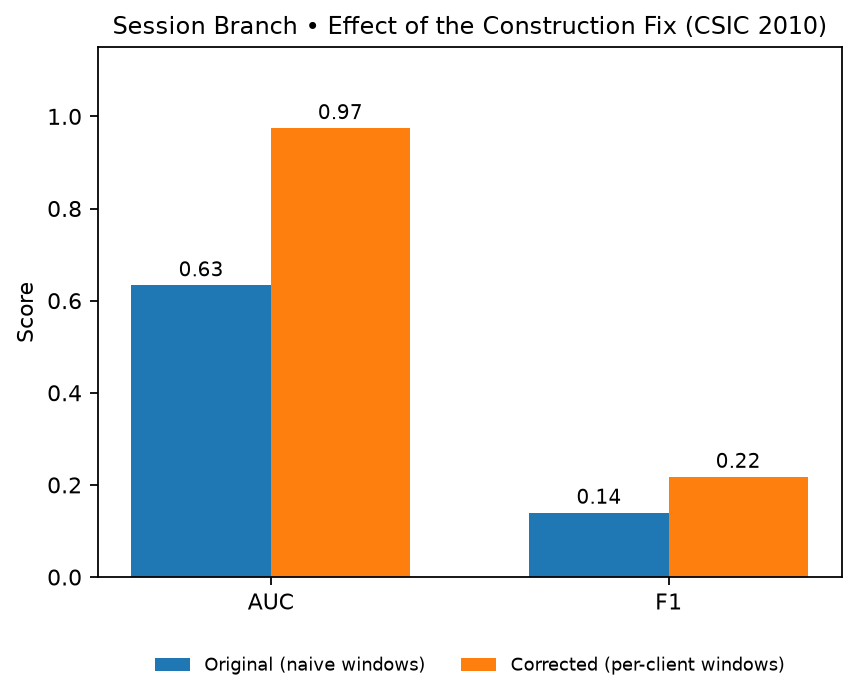
\includegraphics[width=0.6\textwidth]{../artifacts/paper/figures/session_fix_bar.png}
\caption{Session branch AUC and F1 on CSIC 2010, before and after the session construction fix.}
\label{fig:session_fix}
\end{figure}

\subsection{Branch Ablation}

Table~\ref{tab:ablation} reports AUC and F1 for the content, session, and fused branches on every dataset, using the corrected session model throughout. Figure~\ref{fig:heatmap_auc} shows the same AUC values as a heatmap, making it easier to see where each branch does well.

Three structural points about this table explain the pattern in the numbers that follow. First, the content branch scores every request from its own structural features alone (Section~\ref{sec4.4}), so it produces a value on every dataset regardless of session structure, and its AUC differences across datasets reflect differences in how well those structural features separate normal from attack traffic in each dataset, not differences in data volume. Second, the session branch produces a value only where a client sends at least 20 requests in a row (Section~\ref{sec4.5}); as established in Section~\ref{sec5.1}, CSIC~2010 is the only dataset in this study that meets that condition, which is why the session column is populated for one row and blank for the rest. Third, the fused branch reduces to the content branch wherever no session score exists, by the fallback rule given in Section~\ref{sec4.6}, so its AUC only diverges from the content branch's on CSIC~2010, where both branches contribute. AUC is reported here because it is threshold-independent: it reflects how well a branch ranks attacks above normal traffic, not how many alerts a particular percentile threshold would raise, which is the separate question addressed by F1 and the threshold-transfer results in Section~\ref{sec5.4}. Comparing AUC across datasets is still informative, since it shows whether a branch's ranking ability holds up as the traffic changes, but the datasets differ in size, format, and class balance (Table~\ref{tab:datasets}), so an AUC difference between two datasets reflects those differences in the traffic as much as it reflects the model, and should not be read as a controlled comparison.

The content branch reaches a moderate AUC (roughly 0.60--0.70) on most datasets, with high or perfect precision but low recall (roughly 0.06--0.09), because the 95th-percentile threshold only flags the most extreme-looking requests. This matches the precision-first design already used in the original thesis work: fewer, more trustworthy alerts over broad coverage.

The session branch only produces a score on CSIC~2010, for the reason given above. On that dataset it clearly beats the content branch (AUC 0.98 vs. 0.70, both on the held-out split described in Section~\ref{sec5.1}).

The fused branch, on CSIC~2010, sits between the two single branches (AUC 0.77), better than content alone but worse than session alone. On the six datasets without a session score, the fused branch is identical to the content branch, since there is nothing to fuse with. Access Super Long Session 2000 is entirely normal traffic, so its AUC cannot be computed at all (there is only one class), and its F1 is 0 for every branch.

\begin{table}[H]
\caption{Branch ablation: AUC and F1 by dataset, using the corrected session model.}
\label{tab:ablation}
\begin{adjustwidth}{-\extralength}{0cm}
\begin{tabularx}{\fulllength}{lCCCCCC}
\toprule
\textbf{Dataset} & \textbf{Content AUC} & \textbf{Session AUC} & \textbf{Fused AUC} & \textbf{Content F1} & \textbf{Session F1} & \textbf{Fused F1} \\
\midrule
CSIC 2010 (held-out) & 0.70 & 0.98 & 0.76 & 0.11 & 0.12 & 0.11 \\
Access Eval Mix 2000 & 0.69 & --- & 0.69 & 0.11 & --- & 0.11 \\
Access Eval Small 500 & 0.71 & --- & 0.71 & 0.12 & --- & 0.12 \\
Nginx JSON Eval 800 & 0.63 & --- & 0.63 & 0.09 & --- & 0.09 \\
Access Attacks 200 & 0.48 & --- & 0.48 & 0.10 & --- & 0.10 \\
Access Mixed 500 & 0.60 & --- & 0.60 & 0.13 & --- & 0.13 \\
Access Small Benign & 0.63 & --- & 0.63 & 0.17 & --- & 0.17 \\
Access Super Long Session 2000 & n/a & n/a & n/a & 0.00 & 0.00 & 0.00 \\
\bottomrule
\end{tabularx}
{\footnotesize\textit{Note: the CSIC~2010 row is scored on the 32{,}265-row held-out split described in Section~\ref{sec5.1} (7{,}200 benign requests never used to train the session model, plus all 25{,}065 attack requests), not on the full 61{,}065-row file, since the session model is trained on part of CSIC~2010's benign traffic.}\par}
\end{adjustwidth}
\end{table}
\unskip

Table~\ref{tab:ablation} is the main result of this section: it lines up the content, session, and fused branches on every dataset, using the corrected session model throughout. It shows the same pattern described above in numbers: the session column only has values for CSIC~2010, the fused branch matches the content branch exactly wherever no session score exists, and CSIC~2010 is the one row where the session branch clearly leads both other branches.

\begin{figure}[H]
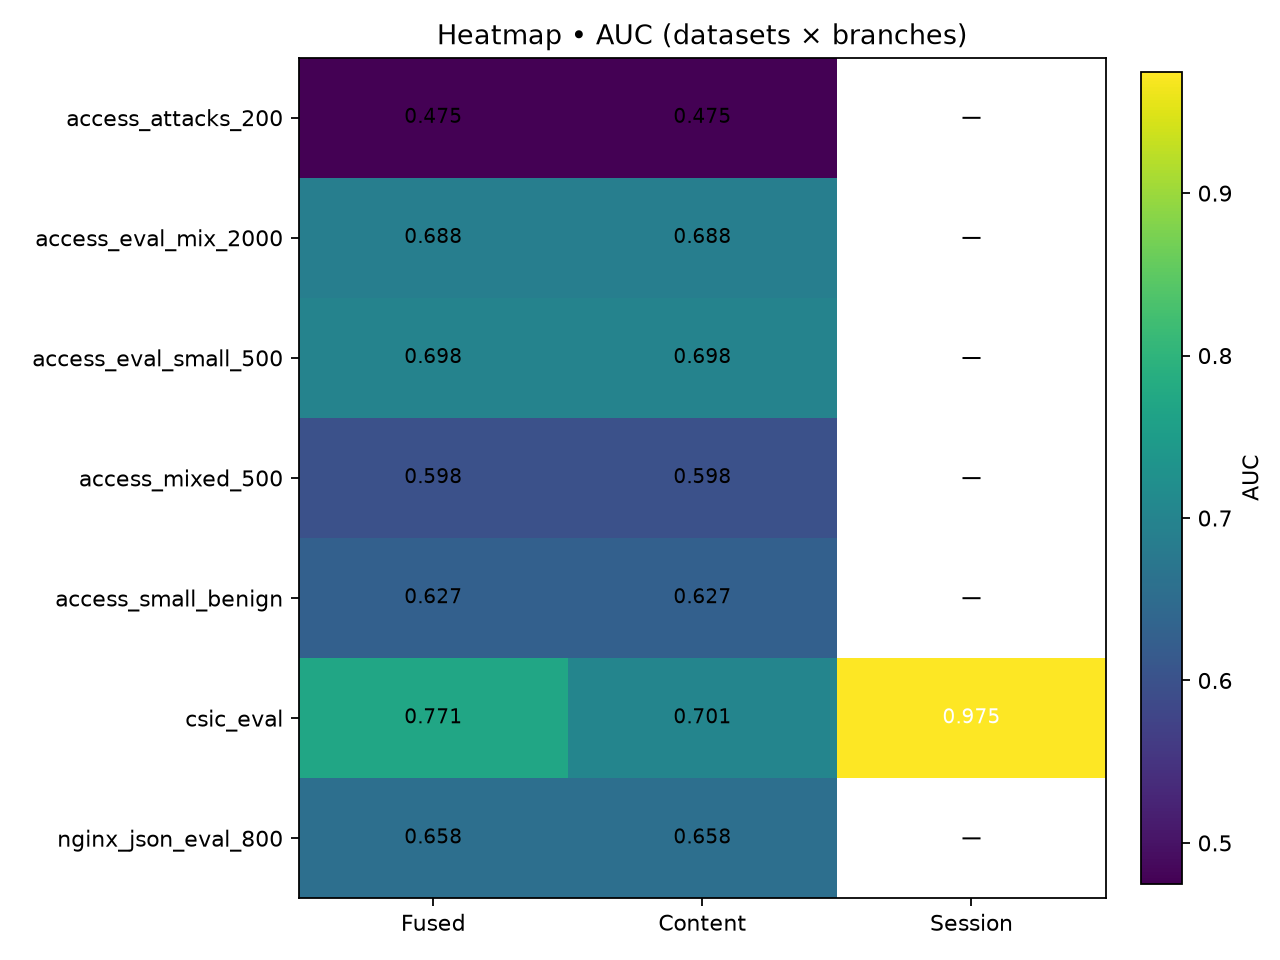
\includegraphics[width=0.72\textwidth]{../artifacts/paper/figures/heatmap_auc.png}
\caption{AUC by dataset and branch (columns left to right: fused, content, session). The session column is blank for every dataset except CSIC~2010, since none of the other datasets has a client with enough consecutive requests to form a valid 20-request session window.}
\label{fig:heatmap_auc}
\end{figure}

Figure~\ref{fig:heatmap_auc} shows the same numbers as Table~\ref{tab:ablation}, laid out as a colour grid with one row per dataset and one column for each branch, where darker cells mean a higher AUC. The session column is empty for every dataset except CSIC~2010, since that is the only dataset where the session branch produces a score at all. The one clearly dark cell in the whole grid is CSIC~2010's session column; the rest of the grid sits in a narrower, more medium range. This makes it easy to see, at a glance, that the session branch's strong result is one bright spot rather than a pattern repeated across datasets.

\subsection{Fusion Weight Sensitivity} \label{sec5.3}

Because a session score only exists for CSIC~2010, this is the only dataset where changing the fusion weight has any effect. Table~\ref{tab:fusion_sweep} sweeps the weight given to each branch in steps of 0.1, from content-only ($w_c=1$) to session-only ($w_s=1$), computed on the same 32{,}265-row held-out split used throughout Section~\ref{sec5.1}.

AUC rises steadily as more weight is put on the session branch, and the best AUC is reached at full session weight, not at any blended point in between, as shown in Figure~\ref{fig:fusion_sweep}. F1, precision, and recall, by contrast, barely move between $w_c=0.5$ and $w_c=0.9$, then step down further at $w_c=1.0$ and jump up only at $w_c=0.0$: the reason is the two branches' raw reconstruction-error scores sit on very different scales at the point that matters for a percentile threshold. At the 95th-percentile cut-off used throughout this paper, the content branch's score is about 89, against about 1.1 for the session branch -- a ratio of roughly 82:1, much larger than the roughly 6:1 ratio at the median. Because fusion is an unweighted average of the two raw scores (Section~\ref{sec4.6}), any $w_c$ of 0.5 or higher leaves the content branch's much larger tail value dominating the fused score numerically, so the \emph{set} of requests that end up above the fused threshold, and hence precision, recall, and F1, stays almost unchanged across that range. AUC keeps moving smoothly across the same range because it depends on the full rank ordering of scores, not just which requests fall above one threshold, so even a small, steadily growing session-branch contribution continues to shift pairwise rankings between mid-scoring requests. This also means the best AUC and the best F1 are both still reached only at full session weight ($w_s=1$): no blended weight beats the session branch alone on raw-score fusion. This goes against the usual assumption that fusing two branches is always better than picking the stronger one, and it further suggests that the unweighted raw-score average is not well matched to the branches' different score scales. On the other seven datasets, sweeping the weight has no effect, since only a content score exists there.

To test whether the scale mismatch itself, rather than fusion as a strategy, is responsible for the flat region above, we recomputed the $w_c=w_s=0.5$ fusion using the normalized combination described in Section~\ref{sec4.6}, on the same held-out CSIC~2010 scores. Mapping each branch onto its own training-score percentile before averaging raises the fused branch's AUC from 0.76 (raw average) to 0.95, much closer to the session branch's own 0.98, and cuts the fused FPR from 0.017 to 0.001, while F1 and precision move in the same direction rather than trading off (F1 0.112~$\rightarrow$~0.120, precision 0.926~$\rightarrow$~0.996). A z-score normalization gives a smaller but still substantial improvement (AUC 0.92). Unlike raw fusion, where only the two extreme weights ($w_c=0$ or $w_c=1$) reach the session branch's own AUC, normalized fusion at an even 0.5/0.5 weight recovers most of that ranking quality while still combining information from both branches. This confirms the diagnosis above: the flat region in Table~\ref{tab:fusion_sweep} is a property of averaging two differently-scaled raw scores, not a property of fusion itself, and score normalization is a cheap, label-free fix that we now recommend over the raw average used elsewhere in this paper's headline numbers, which we keep unchanged so the tables in Section~\ref{sec5} remain directly comparable to the thresholding convention used throughout.

\begin{table}[H]
\caption{Fusion weight sweep on CSIC 2010 (held-out split), in steps of 0.1.}
\label{tab:fusion_sweep}
\begin{tabularx}{\textwidth}{CCCCCCC}
\toprule
\boldmath{$w_c$} & \boldmath{$w_s$} & \textbf{AUC} & \textbf{F1} & \textbf{Precision} & \textbf{Recall} & \textbf{FPR} \\
\midrule
1.0 & 0.0 & 0.70 & 0.109 & 0.925 & 0.058 & 0.016 \\
0.9 & 0.1 & 0.72 & 0.112 & 0.926 & 0.060 & 0.017 \\
0.8 & 0.2 & 0.73 & 0.112 & 0.926 & 0.060 & 0.017 \\
0.7 & 0.3 & 0.74 & 0.112 & 0.926 & 0.060 & 0.017 \\
0.6 & 0.4 & 0.75 & 0.112 & 0.926 & 0.060 & 0.017 \\
0.5 & 0.5 & 0.76 & 0.112 & 0.926 & 0.060 & 0.017 \\
0.4 & 0.6 & 0.77 & 0.113 & 0.932 & 0.060 & 0.015 \\
0.3 & 0.7 & 0.78 & 0.113 & 0.934 & 0.060 & 0.015 \\
0.2 & 0.8 & 0.79 & 0.114 & 0.942 & 0.061 & 0.013 \\
0.1 & 0.9 & 0.82 & 0.116 & 0.955 & 0.062 & 0.010 \\
0.0 & 1.0 & \textbf{0.98} & \textbf{0.121} & \textbf{1.000} & 0.064 & \textbf{0.000} \\
\bottomrule
\end{tabularx}
\end{table}

\begin{figure}[H]
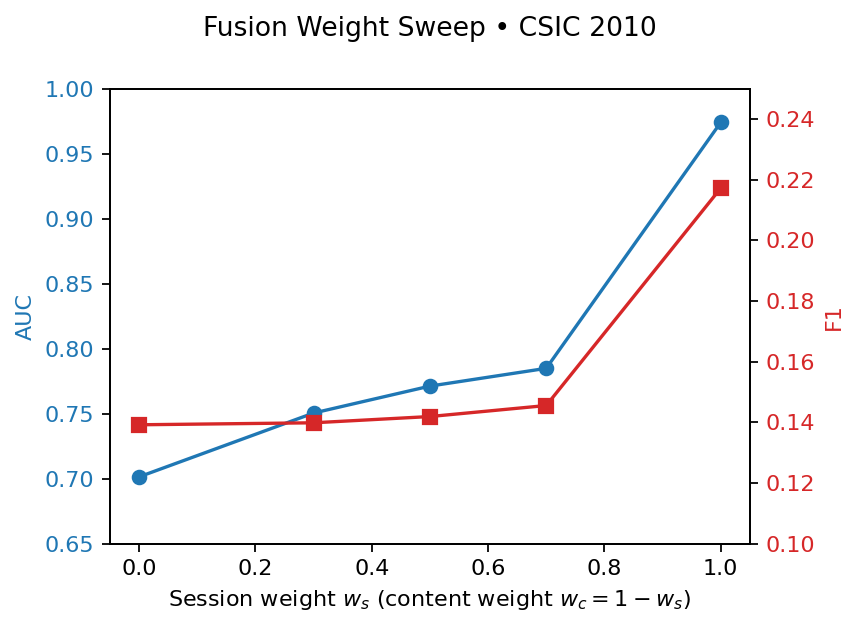
\includegraphics[width=0.6\textwidth]{../artifacts/paper/figures/fusion_sweep_line.png}
\caption{AUC and F1 on CSIC 2010 as the fusion weight shifts from content-only ($w_s=0$) to session-only ($w_s=1$).}
\label{fig:fusion_sweep}
\end{figure}

Figure~\ref{fig:fusion_sweep} shows both the AUC line and the F1 line climbing overall as more weight moves toward the session branch, with F1 flat across the middle of the range for the reason given above and AUC rising throughout. If mixing the two branches ever helped more than using the stronger branch alone, we would expect to see a peak somewhere in the middle of the plot on at least one measure. Instead, both AUC and F1 reach their highest point only at the session-only end. This is the clearest way to see that, for this dataset, blending in the content branch only pulls the score down; it never lifts it above what the session branch reaches on its own.

\subsection{Cross-Dataset Threshold Transfer} \label{sec5.4}

Table~\ref{tab:threshold_transfer} compares the two ways of setting the decision threshold described in Section~\ref{sec4.7}: self-calibrated (tuned separately on each target dataset, using every row in it) and transferred (set once on CSIC~2010's normal traffic only, then applied unchanged). AUC does not change between the two, since AUC does not depend on a threshold; only precision, recall, F1, and false positive rate change.

This result runs counter to what a self-calibrated threshold would be expected to achieve. Using the transferred threshold raises F1 on every target dataset, not by a small amount, but by roughly six to seven times for the fused branch, and by roughly four to five times for the content branch alone. For example, on Access Eval Mix 2000, the fused branch's F1 rises from 0.11 (self-calibrated) to 0.69 (transferred). The same pattern holds on Access Eval Small 500 (0.12 to 0.67) and Nginx JSON Eval 800 (0.09 to 0.65), and at a slightly smaller multiplier for the content branch alone on all three datasets.

The reason is the point already raised in Section~\ref{sec4.2}: these three target datasets are attack-heavy, not normal-heavy (81\%, 79\%, and 78\% attack traffic, respectively). A threshold set at the 95th percentile of a dataset that is mostly attack traffic ends up far too high, since it is really the 95th percentile of a mostly-attack distribution, not a normal-traffic distribution, so it only catches the most extreme 5\% of an already unusual mix. The frozen CSIC threshold, by contrast, is set on genuinely normal traffic, so it sits at a more sensible point and catches far more real attacks, at the cost of a higher false positive rate (up to about 0.16--0.32 on the fused branch, compared to 0.00--0.05 self-calibrated).

In practice, this shows that on these datasets, what data a threshold is calibrated on matters more than whether it is calibrated on the same dataset being tested. A threshold set on real normal traffic, even from a completely different dataset, can work better than one set on the target dataset itself, if that target dataset does not actually represent normal conditions well. Figure~\ref{fig:threshold_transfer} shows the self-calibrated and transferred F1 scores side by side for both branches.

\begin{table}[H]
\caption{Self-calibrated vs. transferred threshold, on the three target datasets.}
\label{tab:threshold_transfer}
\begin{adjustwidth}{-\extralength}{0cm}
\begin{tabularx}{\fulllength}{llCCCCCC}
\toprule
\textbf{Target Dataset} & \textbf{Branch} & \textbf{AUC} & \textbf{Self F1} & \textbf{Self FPR} & \textbf{Transf. F1} & \textbf{Transf. Recall} & \textbf{Transf. FPR} \\
\midrule
Access Eval Mix 2000 & Content & 0.69 & 0.11 & 0.02 & 0.50 & 0.34 & 0.04 \\
Access Eval Mix 2000 & Fused & 0.69 & 0.11 & 0.02 & 0.69 & 0.55 & 0.24 \\
Access Eval Small 500 & Content & 0.71 & 0.12 & 0.00 & 0.48 & 0.31 & 0.00 \\
Access Eval Small 500 & Fused & 0.71 & 0.12 & 0.00 & 0.67 & 0.52 & 0.16 \\
Nginx JSON Eval 800 & Content & 0.63 & 0.09 & 0.05 & 0.45 & 0.30 & 0.11 \\
Nginx JSON Eval 800 & Fused & 0.63 & 0.09 & 0.05 & 0.65 & 0.53 & 0.32 \\
\bottomrule
\end{tabularx}
\end{adjustwidth}
\end{table}
\unskip

\begin{figure}[H]
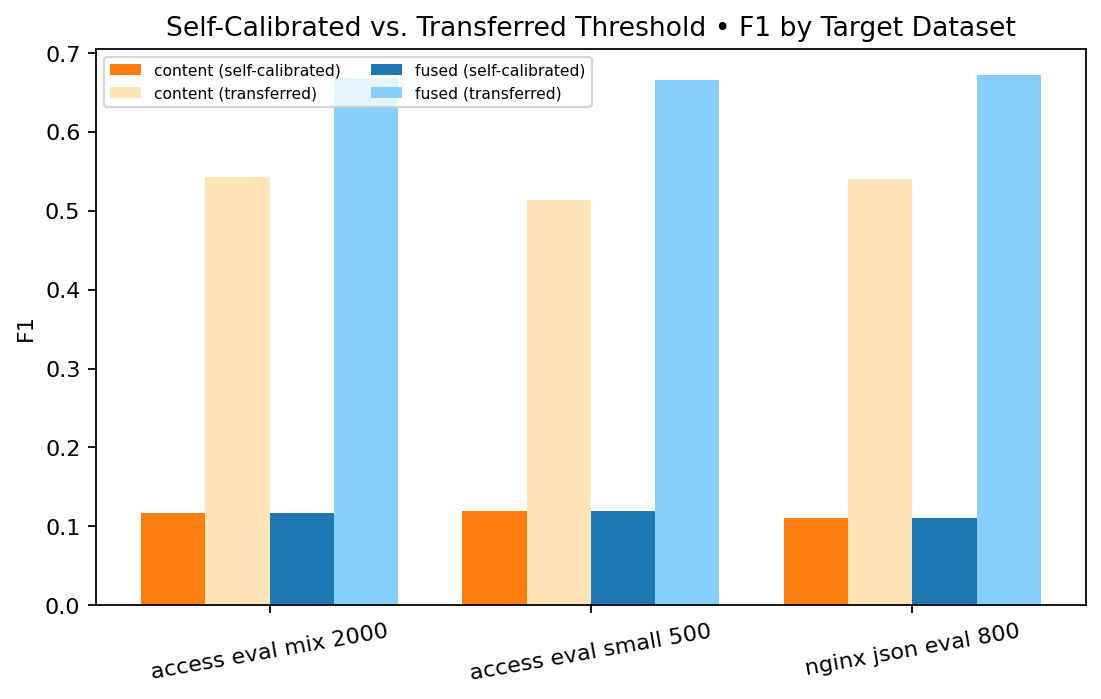
\includegraphics[width=0.72\textwidth]{../artifacts/paper/figures/threshold_transfer_bar.png}
\caption{Self-calibrated vs.\ transferred-threshold F1, content and fused branches, by target dataset.}
\label{fig:threshold_transfer}
\end{figure}

Figure~\ref{fig:threshold_transfer} places the self-calibrated and transferred F1 scores side by side for each target dataset, for both the content and fused branches. In every pair of bars, the transferred-threshold bar is much taller than the self-calibrated bar next to it, across all three datasets and both branches. This makes the size of the improvement easy to see at a glance: it is not a small edge in one or two cases, it is a large, consistent jump everywhere this comparison is made.

\subsection{Comparison with Classical Baselines} \label{sec5.5}

Table~\ref{tab:baselines} compares our content and fused branches with three classical baselines: Random Forest, which is trained using attack labels, unlike our own models, and Isolation Forest and One-Class SVM, which are trained only on normal traffic, the same setup as our own models.

Random Forest usually reaches the highest AUC of all methods (for example, 0.90 on Access Attacks 200 and 0.89 on CSIC~2010), which is expected, since it is the only method here allowed to see attack labels during training. Its F1 score is also high, but this comes with a much higher false positive rate than our fused branch in every case (for example, 0.55 on Access Eval Mix 2000, compared to 0.00 for our fused branch on the same dataset). This trade-off matters in a real security setting, where too many false alerts can make a system less useful even when its raw detection rate looks strong.

Isolation Forest and One-Class SVM, which do not use attack labels, generally score lower than Random Forest on AUC, but their comparison against our own branches is mixed, and Table~\ref{tab:bootstrap_ci} shows that most of these dataset-level differences are not distinguishable from sampling noise at the sample sizes available here. To check this, we computed 2{,}000-resample bootstrap 95\% confidence intervals for AUC directly from the per-request scores already saved for every method (Table~\ref{tab:bootstrap_ci}); several of the datasets in Table~\ref{tab:baselines} have as few as 24 to 160 rows in a baseline's 20\% held-out test fold, so a single point-estimate comparison there is not reliable on its own. Two comparisons are clear once uncertainty is accounted for: on CSIC~2010, the fused branch's interval (0.755--0.770) does not overlap either unsupervised baseline's (Isolation Forest 0.703--0.721, One-Class SVM 0.437--0.458), so the fused branch is reliably ahead there; and on Access Attacks 200, both Random Forest (0.769--0.995) and Isolation Forest (0.724--0.972) sit clearly above the fused branch (0.385--0.560), so that loss is real rather than noise. On the other five datasets, the fused branch's interval overlaps at least one classical baseline's interval, meaning the point-estimate "wins" and "losses" reported for those datasets (for example, 0.60 vs. 0.64 on Access Mixed 500) are not statistically distinguishable given the sample sizes involved, and we no longer describe them as the fused branch "beating" or "losing to" a specific baseline. The one dataset where our system does clearly best of all methods, including Random Forest, is CSIC~2010, where the session branch alone reaches an AUC of 0.98 (Table~\ref{tab:ablation}), higher than every method or baseline listed in Table~\ref{tab:baselines}, which does not include a session column since the session branch produces no score on the other datasets there. Figure~\ref{fig:baseline_auc} plots all five methods' AUC side by side across every dataset.

\begin{table}[H]
\caption{Comparison with classical baselines.}
\label{tab:baselines}
\begin{adjustwidth}{-\extralength}{0cm}
\begin{tabularx}{\fulllength}{lCCCCCCC}
\toprule
\textbf{Dataset} & \textbf{Content AUC} & \textbf{Fused AUC} & \textbf{Fused FPR} & \textbf{RF AUC} & \textbf{RF FPR} & \textbf{IForest AUC} & \textbf{OCSVM AUC} \\
\midrule
CSIC 2010 (held-out) & 0.70 & 0.76 & 0.02 & 0.89 & 0.30 & 0.71 & 0.45 \\
Access Eval Mix 2000 & 0.69 & 0.69 & 0.02 & 0.78 & 0.55 & 0.66 & 0.62 \\
Access Eval Small 500 & 0.71 & 0.71 & 0.00 & 0.75 & 0.58 & 0.66 & 0.66 \\
Nginx JSON Eval 800 & 0.63 & 0.63 & 0.05 & 0.68 & 0.62 & 0.55 & 0.55 \\
Access Attacks 200 & 0.48 & 0.48 & 0.03 & 0.90 & 0.20 & 0.86 & 0.61 \\
Access Mixed 500 & 0.60 & 0.60 & 0.02 & 0.68 & 0.44 & 0.57 & 0.64 \\
Access Small Benign & 0.63 & 0.63 & 0.00 & 0.72 & 0.25 & 0.76 & 0.47 \\
\bottomrule
\end{tabularx}
{\footnotesize\textit{Note: Fused FPR is the fused branch's own false-positive rate at its 95th-percentile threshold, included so the false-positive-rate comparison made in Section~\ref{sec6} can be checked directly against this table. The CSIC~2010 row uses the same 32{,}265-row held-out split as Tables~\ref{tab:session_fix}--\ref{tab:fusion_sweep} for the content and fused branches; RF, IForest, and OCSVM are each evaluated on their own 20\% held-out split of the full 61{,}065-row file (Section~\ref{sec4.9}), so the sample sizes across columns are not identical, though none of the methods compared here is evaluated on any of its own training data.}\par}
\end{adjustwidth}
\end{table}
\unskip

\begin{table}[H]
\caption{Bootstrap 95\% confidence intervals for AUC (2{,}000 resamples), fused branch vs.\ classical baselines.}
\label{tab:bootstrap_ci}
\begin{adjustwidth}{-\extralength}{0cm}
\begin{tabularx}{\fulllength}{lCCCC}
\toprule
\textbf{Dataset} & \textbf{Fused AUC [95\% CI]} & \textbf{RF AUC [95\% CI]} & \textbf{IForest AUC [95\% CI]} & \textbf{OCSVM AUC [95\% CI]} \\
\midrule
CSIC 2010 & 0.762 [0.755, 0.770] & 0.893 [0.888, 0.899] & 0.712 [0.703, 0.721] & 0.448 [0.437, 0.458] \\
Access Eval Mix 2000 & 0.692 [0.665, 0.717] & 0.776 [0.728, 0.819] & 0.664 [0.597, 0.729] & 0.621 [0.562, 0.681] \\
Access Eval Small 500 & 0.714 [0.669, 0.760] & 0.754 [0.653, 0.852] & 0.659 [0.530, 0.778] & 0.662 [0.541, 0.777] \\
Nginx JSON Eval 800 & 0.625 [0.579, 0.674] & 0.677 [0.593, 0.760] & 0.548 [0.436, 0.660] & 0.553 [0.447, 0.657] \\
Access Attacks 200 & 0.475 [0.385, 0.560] & 0.900 [0.769, 0.995] & 0.862 [0.724, 0.972] & 0.610 [0.389, 0.811] \\
Access Mixed 500 & 0.599 [0.551, 0.646] & 0.679 [0.576, 0.779] & 0.568 [0.454, 0.676] & 0.634 [0.526, 0.739] \\
Access Small Benign & 0.628 [0.525, 0.724] & 0.727 [0.489, 0.929] & 0.759 [0.531, 0.936] & 0.474 [0.222, 0.711] \\
\bottomrule
\end{tabularx}
{\footnotesize\textit{Note: the fused branch's interval is computed on the same sample used for its point estimate in Table~\ref{tab:baselines} (the dataset's full evaluation file, or the held-out split of Section~\ref{sec5.1} for CSIC~2010); each baseline's interval is computed on that baseline's own 20\% held-out test fold (Section~\ref{sec4.9}), which is as small as 24--160 rows for the self-generated datasets. Bold takeaway: only the CSIC~2010 and Access Attacks 200 comparisons are outside overlapping intervals; every other dataset's fused-vs-baseline point-estimate difference sits within the two methods' combined sampling uncertainty.}\par}
\end{adjustwidth}
\end{table}
\unskip

\begin{figure}[H]
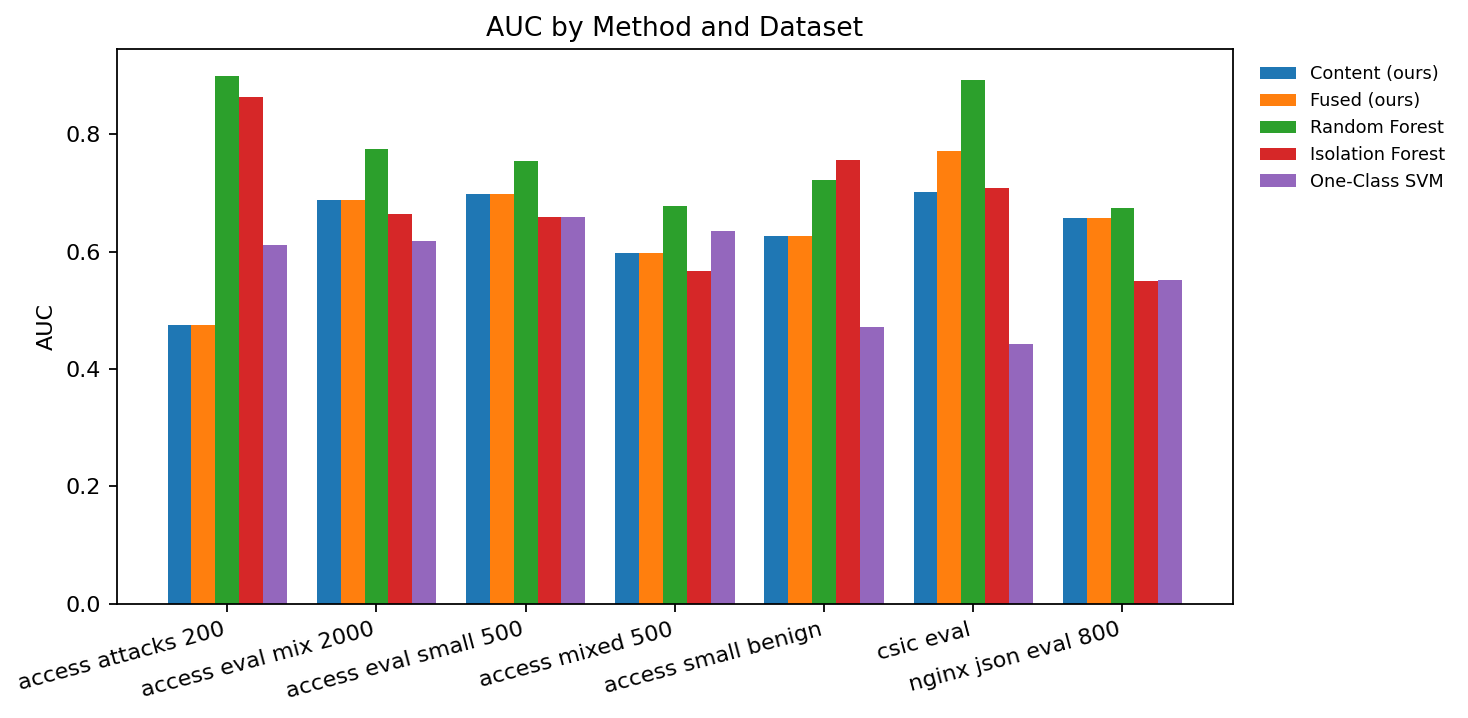
\includegraphics[width=\textwidth]{../artifacts/paper/figures/baseline_auc_bar.png}
\caption{AUC by method and dataset: our content and fused branches against Random Forest, Isolation Forest, and One-Class SVM.}
\label{fig:baseline_auc}
\end{figure}

Figure~\ref{fig:baseline_auc} lines up all five methods' AUC scores side by side for every dataset, so the pattern in Table~\ref{tab:baselines} can be seen directly. Random Forest's bar is usually the tallest, since it is the only method trained with attack labels. Our fused branch's bar is taller than both Isolation Forest's and One-Class SVM's on most datasets, but Table~\ref{tab:bootstrap_ci} shows that only the CSIC~2010 gap is large enough to be distinguishable from sampling noise; the fused branch is clearly shorter than both on Access Attacks 200, where Isolation Forest's bar is noticeably taller than ours and the gap is confirmed by non-overlapping confidence intervals.

\subsection{Inference Speed} \label{sec5.6}

We also measured how fast the system runs, using the Access Eval Mix 2000 log. Scoring one request at a time, as a live system would, the content branch takes about 0.14~ms per request on average, and the session branch about 0.08~ms, giving an overall throughput of about 4{,}420 requests per second. Scoring in batches instead, the same log runs at about 630{,}000 lines per second, roughly 140 times faster than one-at-a-time scoring. Both numbers are fast enough for near-real-time use on ordinary hardware, with batch scoring far ahead whenever requests can be grouped before scoring.

\subsection{Training-Run Variance} \label{sec5.7}

All results reported so far come from a single training run per model, using the fixed seed noted in Section~\ref{sec4}. To check whether these point estimates are representative rather than a single favourable run, we retrained both the content and session branches from scratch five times, using five different random seeds, and re-evaluated every retrained pair on all seven labelled datasets. Table~\ref{tab:seed_variance} reports the resulting AUC as a mean $\pm$ one standard deviation across the five runs.

\begin{table}[H]
\caption{AUC across five independently trained models per branch (mean $\pm$ standard deviation, 5 seeds).}
\label{tab:seed_variance}
\begin{adjustwidth}{-\extralength}{0cm}
\begin{tabularx}{\fulllength}{lCCC}
\toprule
\textbf{Dataset} & \textbf{Content AUC} & \textbf{Session AUC} & \textbf{Fused AUC} \\
\midrule
CSIC 2010 (held-out) & 0.699 $\pm$ 0.000 & 0.972 $\pm$ 0.010 & 0.760 $\pm$ 0.003 \\
Access Eval Mix 2000 & 0.692 $\pm$ 0.001 & --- & 0.692 $\pm$ 0.001 \\
Access Eval Small 500 & 0.713 $\pm$ 0.000 & --- & 0.713 $\pm$ 0.000 \\
Nginx JSON Eval 800 & 0.626 $\pm$ 0.001 & --- & 0.626 $\pm$ 0.001 \\
Access Attacks 200 & 0.476 $\pm$ 0.002 & --- & 0.476 $\pm$ 0.002 \\
Access Mixed 500 & 0.598 $\pm$ 0.002 & --- & 0.598 $\pm$ 0.002 \\
Access Small Benign & 0.627 $\pm$ 0.001 & --- & 0.627 $\pm$ 0.001 \\
\bottomrule
\end{tabularx}
\end{adjustwidth}
{\footnotesize\textit{Note: each row is computed from five independently initialised and trained models (content and session branches retrained together per seed), not five resamples of one trained model's scores, so this captures training-time variance in addition to the evaluation-sampling variance already reported in Table~\ref{tab:bootstrap_ci}. Session AUC is reported only for CSIC~2010, the one dataset with real session structure (Section~\ref{sec5.1}).}\par}
\end{table}
\unskip

The variance is small everywhere, and smallest exactly where it matters most for this paper's headline claim: the session branch's AUC on CSIC~2010 is $0.972 \pm 0.010$ across five independently trained models, so the single-run figure of 0.98 used throughout Section~\ref{sec5} sits well within one standard deviation of the five-run mean, not at an unrepresentative extreme. The content branch's AUC varies even less (standard deviation at or below 0.002 on every dataset) despite the five models having verifiably different learned weights (confirmed by comparing model checkpoints directly), which suggests the small feed-forward autoencoder converges to a similar solution regardless of initialisation, at least at the scale of training data used here. This does not substitute for testing on additional session-rich datasets, which would test whether the finding generalises to different traffic rather than whether it is stable under retraining, but it does rule out the specific concern that the reported session-branch improvement could be an artefact of one favourable random initialisation.

\subsection{Summary of Results}

Taken together, these results show three things. First, the session branch is powerful, but only where the traffic actually contains real client sessions; the fix in Section~\ref{sec4.5} changes its usefulness from close to a coin flip to strong detection on the one dataset, CSIC~2010, where it can genuinely operate. Second, fusion is not automatically better than picking the stronger branch: on CSIC~2010, weighting fully toward the session branch beats every blended fusion weight tested. Third, how a threshold is set matters as much as which model produces the score: a threshold frozen from real normal traffic, even from a different dataset, outperformed a threshold tuned on the target dataset itself, because several of the target datasets used here are attack-heavy rather than normal-heavy.

\section{Discussion} \label{sec6}

The results in Section~\ref{sec5} support the case, made in Section~\ref{sec1}, that content-based and behaviour-based detection are complementary rather than interchangeable, but they also complicate the usual assumption that combining the two is always the better choice. Prior hybrid, fusion-based work has generally reported that combining detection signals improves over any single-model detector~\cite{kamal2025}, and the session branch here does exactly what that line of work would predict on CSIC~2010, comfortably outperforming the content branch alone once its session windows are built correctly. What the fusion-weight sweep in Table~\ref{tab:fusion_sweep} shows, however, is that blending the two branches on that same dataset is strictly worse than using the session branch on its own: every mixed weight tested sits between the two single-branch scores, and the best result is at full session weight. This is not a contradiction of the hybrid-detection literature so much as a boundary condition on it -- fusion helps when the two branches make comparably reliable but different mistakes, and it hurts when one branch is reliably much stronger than the other on the traffic being scored, since averaging then just pulls the fused score toward the weaker signal. A fixed 50/50 weighting, of the kind used as a sensible default in the absence of other information, is therefore not a safe assumption to carry into a new dataset without checking it. Section~\ref{sec5.3} traces this specifically to the two branches' raw reconstruction-error scores sitting on very different numeric scales (roughly 82:1 at the operating threshold), and shows that normalizing each branch against its own training-score distribution before averaging, rather than abandoning fusion altogether, recovers most of the session branch's ranking quality (AUC 0.95 vs.\ 0.98) while still combining both signals -- so the boundary condition above is a property of unweighted raw-score fusion specifically, not of combining the two branches in general.

The session-branch results also speak directly to the caveat raised about behaviour-based detection in Section~\ref{sec3}: a sequence model can only model a sequence if one actually exists in the data. The correction described in Section~\ref{sec4.5} is a straightforward bug fix -- windows should never mix requests from different clients -- but its effect size (AUC rising from 0.63 to 0.98 on CSIC~2010's held-out split) shows how badly a session model can be misled by session windows that are not really sessions at all. The other side of that same fix is that six of the eight datasets used here have essentially no client with 20 or more requests to build a window from, so the corrected model produces no score on them whatsoever. This is a genuine limitation of session-based detection as a technique, not an artefact of this particular implementation, and it means that a deployment decision about whether to run a session branch at all should be based on measuring the client request-count distribution of the target traffic first, rather than assumed to be generally useful the way the content branch is.

It is worth being precise about what "cross-dataset generalisation" means in this study, since two different results are sometimes read as supporting the same claim. The content branch's own ranking ability, its AUC, is measured independently on all eight datasets (Table~\ref{tab:ablation}), including the seven the model was never trained or threshold-calibrated on in any way; the fact that its AUC stays in a broadly similar 0.48--0.71 range across log formats as different as Apache Combined, Apache Common, and structured JSON is evidence of \emph{model generalisation} -- the learned reconstruction behaviour transfers to unseen traffic shapes without retraining. The threshold-transfer result discussed next is a separate claim about \emph{threshold generalisation}: it shows that a decision boundary calibrated once on CSIC~2010 still works, and in fact works better, when applied unchanged to three other datasets, which says nothing by itself about how well the underlying score ranks attacks on those datasets. The two results are complementary but not interchangeable, and the rest of this section keeps them distinct rather than treating both as instances of one generalisation claim.

The cross-dataset threshold-transfer result in Table~\ref{tab:threshold_transfer} is the most counter-intuitive finding in this study. A percentile threshold is only a meaningful proxy for "unusually different from normal traffic" if the distribution it is computed on is itself mostly normal traffic. Three of the target datasets used here are between 78\% and 81\% attack traffic (Section~\ref{sec4.2}), so a threshold set at their 95th percentile is really being set against a distribution made up mostly of attack scores, not mostly normal scores. This pushes the threshold far higher than it would be on real normal traffic, since it has to sit above a large share of already-high attack scores rather than just the tail end of normal behaviour, which is why recall and F1 are so low in the self-calibrated columns of Table~\ref{tab:threshold_transfer}. This is consistent with the broader finding in the cross-dataset generalisation literature that a fixed evaluation protocol can hide large differences in how well a threshold transfers~\cite{cantone2024}, but the direction of the effect here is the opposite of the usual warning: instead of a model looking better than it really is because it was tuned on its own test data, the self-calibrated approach makes the framework look far \emph{worse} than it is, because the calibration data was not the kind of traffic a percentile threshold assumes. The practical implication is that a percentile threshold should be calibrated on traffic that is known, or at least believed with reasonable confidence, to be predominantly normal, even if that traffic comes from a different source than the traffic being monitored, rather than calibrated automatically on whatever traffic happens to be available at deployment time.

Against the classical baselines, the pattern in Table~\ref{tab:baselines} reinforces a point made in Section~\ref{sec4.7} about what this framework is optimised for. Random Forest reaches the highest AUC in most cases, which is unsurprising given it is the only method trained with attack labels, but it does so with a much higher false positive rate than the fused branch on every dataset compared: the fused branch's own FPR is no higher than 0.05 on any of the seven datasets, exactly 0.00 on two of them (Access Eval Small 500 and Access Small Benign, Table~\ref{tab:baselines}), while Random Forest's false positive rate ranges from 0.20 to 0.62. This comparison should be read with the evaluation-protocol difference noted in Section~\ref{sec4.9} in mind: the classical baselines are each scored on their own 20\% held-out fold of a dataset, while the content, session, and fused branches are scored on the dataset's full evaluation file (or, for CSIC~2010, on the disjoint held-out split of Section~\ref{sec5.1}), so the two sides of each row are not evaluated on identically sized or composed samples, even though neither side is scored on its own training data. In a real deployment, false positives carry a direct operational cost -- alerts that must be triaged by a human -- so a detector with a lower AUC but a substantially lower false-positive rate is not automatically the worse choice, particularly for a semi-supervised setting where attack labels are assumed unavailable in the first place. The unsupervised baselines (Isolation Forest, One-Class SVM) are a fairer comparison, since they share the same no-attack-label constraint as this framework. Against these, the bootstrap confidence intervals in Table~\ref{tab:bootstrap_ci} show the fused branch is reliably ahead on only one dataset, CSIC~2010, and reliably behind on only one, Access Attacks 200, where Isolation Forest is the stronger method; on the remaining five datasets the point-estimate differences between the fused branch and one or both unsupervised baselines fall inside overlapping confidence intervals, so we do not treat them as established wins or losses at the sample sizes available here. Combined with the inference-speed results in Section~\ref{sec5}, which show the framework comfortably meets near-real-time throughput requirements, this suggests the precision-first design carried over from the original thesis work (Section~\ref{sec4}) is a reasonable operating point for a system meant to generate trustworthy rather than exhaustive alerts.

This study has several limitations that should temper how far its findings are generalised. First, the session branch's strong result is demonstrated on only one dataset, CSIC~2010, because it is the only dataset in this study with enough per-client requests to build real session windows; the claim that a corrected session model helps is well supported where it applies, but it has not been shown to help on genuinely session-rich traffic of a different shape or scale. Second, several of the self-generated datasets are small (as few as 120 to 500 requests), which limits the statistical precision of the metrics computed on them and means single-point AUC and F1 differences between datasets should be read as indicative rather than tightly bounded. Third, the 11-feature representation (Table~\ref{tab:features}) is deliberately structural and does not inspect request bodies or query values directly, so it is unlikely to catch attacks whose payload is anomalous but whose structural shape (method, path length, status code, response size) looks unremarkable; this is a deliberate scope choice rather than an oversight, but it bounds what the content branch can be expected to catch. Fourth, the self-generated attack traffic was produced with a small number of well-known tools (sqlmap and nikto), so it may not represent the full diversity of real-world attack techniques or evasion strategies. Fifth, the headline numbers in Section~\ref{sec5} are reported from a single training run per configuration, using the fixed random seed noted in Section~\ref{sec4}; Section~\ref{sec5.7} addresses whether this single run is representative by retraining every branch five times from independent random seeds and reporting the resulting AUC variance (Table~\ref{tab:seed_variance}). Training-time variance turns out to be small everywhere, including for the session-branch result on CSIC~2010 that this limitation previously singled out, so the reported figures are not an artefact of one favourable initialisation; this is a narrower claim than cross-dataset generalisation, however, and does not substitute for testing on session-rich traffic beyond CSIC~2010 (First, above). We also computed bootstrap 95\% confidence intervals for the AUC comparisons against the classical baselines (Table~\ref{tab:bootstrap_ci}), since these do not require retraining and capture evaluation-sampling variance rather than training variance, and the intervals show that most of the seven-dataset, point-estimate "wins" and "losses" against Isolation Forest and One-Class SVM discussed in Section~\ref{sec5.5} are not statistically distinguishable at the sample sizes available -- several baseline test folds have fewer than 200 rows -- so those comparisons should be read as indicative rather than settled, and only the CSIC~2010 and Access Attacks 200 comparisons are large enough to treat as established. Sixth, all evaluation here is offline, on fixed logs; the inference-speed measurements in Section~\ref{sec5} indicate the framework's computational profile is compatible with real-time use, but the framework has not actually been run against a live traffic stream, so behaviour under real deployment conditions such as concept drift or partially arriving sessions remains untested.

These limitations point to concrete future work. Testing the corrected session model on additional datasets with genuine, larger-scale multi-request sessions would show whether the CSIC~2010 result generalises or is specific to that dataset's traffic pattern; a concrete candidate is Biblio-US17, a recently published, real-world, labelled HTTP log dataset (47 million requests, six months of traffic from a university library website)~\cite{diazverdejo2025}, though its public field list would need to be confirmed to include the per-client identifiers this framework's session branch requires before it could be used for this purpose. Extending the feature representation to include lightweight payload or query-string signals, without giving up the efficiency of the current structural features, could let the content branch catch attacks that do not alter a request's structural shape. Because the threshold-transfer result depends entirely on how "normal enough to calibrate on" is judged, an adaptive or likelihood-based thresholding scheme that estimates its own confidence in the calibration data, rather than assuming a fixed percentile is always appropriate, is a natural next step. Finally, validating the framework against live or replayed traffic, and evaluating it against a wider and more current set of attack tools, would test the real-time and generalisation claims made here under conditions closer to genuine deployment.

\section{Conclusions} \label{sec7}

This paper presented a hybrid anomaly detection framework for web server logs that fuses a content-based autoencoder, which scores individual HTTP requests on their structural features, with a session-based variational LSTM autoencoder, which scores genuine per-client request sequences, and evaluated it across eight datasets in three log formats, under both branch-ablation and cross-dataset threshold-transfer protocols, rather than the single-dataset evaluations common in this literature (Section~\ref{sec3}).

Three findings stand out. Correcting a session-construction fault that had mixed different clients' requests into the same window raised the session branch's AUC on CSIC~2010 from 0.63 to 0.98, evaluated on a held-out split of client traffic never used to train the corrected model, but the corrected model produced no score on the six datasets that lack real multi-request client sessions, so a session branch is only as useful as the session structure present in the traffic being scored. Fusing the two branches is not automatically better than using the stronger one alone: on CSIC~2010, weighting fully toward the session branch beat every blended weight tested. A threshold calibrated once on normal CSIC~2010 traffic and transferred unchanged to three attack-heavy datasets raised fused F1 six- to seven-fold over a threshold tuned separately on each dataset (for example, 0.11 to 0.69 on Access Eval Mix 2000), because those datasets contain too much attack traffic for self-calibration to represent normal behaviour. Alongside these findings, the framework achieved a lower false-positive rate than a labelled Random Forest baseline on every dataset compared, and processed requests fast enough for near-real-time use, at roughly 630{,}000 lines per second in batch mode; bootstrap confidence intervals on the AUC comparisons against the unsupervised Isolation Forest and One-Class SVM baselines (Table~\ref{tab:bootstrap_ci}) show the fused branch reliably ahead on CSIC~2010 and reliably behind on Access Attacks 200, with the remaining five dataset-level differences too small, relative to sample size, to call either way.

The practical implication is that, in fusion-based web-log anomaly detection, how session windows are built and how thresholds are calibrated can matter as much as which model architecture is used, and both should be checked explicitly for a given deployment rather than assumed to transfer safely from one dataset to another.

The main limitations are that only one dataset in this study has genuine session structure to demonstrate the session branch's benefit on, the feature representation is structural rather than payload-aware, and all evaluation is on offline logs rather than live traffic (Section~\ref{sec6}). Future work should test the corrected session model on additional session-rich datasets, extend the feature representation to lightweight payload signals, develop an adaptive thresholding scheme that can judge how normal its own calibration data is, and validate the framework against live or replayed traffic.

\vspace{6pt}

\authorcontributions{A.R.:~Conceptualization, Methodology, Software, Validation, Formal Analysis, Investigation, Data Curation, Writing---Original Draft Preparation, Writing---Review and Editing, Visualisation. M.N.:~Conceptualization, Validation, Writing---Review and Editing, Supervision, Project Administration. M.H.:~Conceptualization, Validation, Writing---Review and Editing, Supervision. All authors have read and agreed to the published version of the manuscript.}

\funding{This work received no external funding.}

\institutionalreview{Not applicable. This research did not involve human participants or animals. The self-generated traffic logs were produced against a test application built for this study, and the CSIC~2010 dataset is a pre-existing, publicly available dataset.}

\informedconsent{Not applicable.}

\dataavailability{The CSIC~2010 HTTP dataset is publicly available from the Information Security Institute of CSIC (Spanish National Research Council). The self-generated Apache- and Nginx-style log datasets, together with the trained models, scalers, and score outputs used to produce the results in Section~\ref{sec5}, are available from the corresponding author upon reasonable request.}

\acknowledgments{The University of the West of Scotland is thanked for providing the academic environment and computational facilities for conducting this research. The authors also thank their supervisors for their guidance and constructive feedback throughout this work.}

\conflictsofinterest{The authors declare no conflicts of interest.}

\abbreviations{Abbreviations}{
The following abbreviations are used in this manuscript:\\

\noindent
\begin{tabular}{@{}ll}
HTTP & Hypertext Transfer Protocol\\
IDS/IPS & Intrusion Detection/Prevention System\\
LSTM & Long Short-Term Memory\\
VAE & Variational Autoencoder\\
KL & Kullback--Leibler (divergence)\\
AE & Autoencoder\\
ROC & Receiver Operating Characteristic\\
AUC & Area Under the Curve\\
PR & Precision--Recall\\
F1 & F1 Score (harmonic mean of precision and recall)\\
FPR & False Positive Rate\\
RF & Random Forest\\
SVM & Support Vector Machine\\
OCSVM & One-Class Support Vector Machine\\
JSON & JavaScript Object Notation\\
API & Application Programming Interface
\end{tabular}
}

%=================================================================
\begin{adjustwidth}{-\extralength}{0cm}
\reftitle{References}
\begin{thebibliography}{999}

\bibitem[Scarfone and Mell(2007)]{scarfone2007}
Scarfone, K.; Mell, P. \emph{Guide to Intrusion Detection and Prevention Systems (IDPS)}; NIST Special Publication 800-94; National Institute of Standards and Technology: Gaithersburg, MD, USA, 2007. \url{https://doi.org/10.6028/NIST.SP.800-94}.

\bibitem[Chandola et al.(2009)]{chandola2009}
Chandola, V.; Banerjee, A.; Kumar, V. Anomaly detection: A survey. \emph{ACM Comput. Surv.} \textbf{2009}, \emph{41}, 15. \url{https://doi.org/10.1145/1541880.1541882}.

\bibitem[Hochreiter and Schmidhuber(1997)]{hochreiter1997}
Hochreiter, S.; Schmidhuber, J. Long Short-Term Memory. \emph{Neural Comput.} \textbf{1997}, \emph{9}, 1735--1780. \url{https://doi.org/10.1162/neco.1997.9.8.1735}.

\bibitem[Nedelkoski et al.(2020)]{nedelkoski2020}
Nedelkoski, S.; Bogatinovski, J.; Acker, A.; Cardoso, J.; Kao, O. Self-Attentive Classification-Based Anomaly Detection in Unstructured Logs. In Proceedings of the 2020 IEEE International Conference on Data Mining (ICDM), Sorrento, Italy, 17--20 November 2020; pp. 1196--1201. \url{https://arxiv.org/abs/2008.09340}.

\bibitem[Du et al.(2017)]{du2017}
Du, M.; Li, F.; Zheng, G.; Srikumar, V. DeepLog: Anomaly Detection and Diagnosis from System Logs through Deep Learning. In Proceedings of the 2017 ACM SIGSAC Conference on Computer and Communications Security (CCS), Dallas, TX, USA, 30 October--3 November 2017; pp. 1285--1298. \url{https://doi.org/10.1145/3133956.3134015}.

\bibitem[Kingma and Welling(2014)]{kingma2014}
Kingma, D.P.; Welling, M. Auto-Encoding Variational Bayes. In Proceedings of the 2nd International Conference on Learning Representations (ICLR), Banff, AB, Canada, 14--16 April 2014. \url{https://arxiv.org/abs/1312.6114}.

\bibitem[An and Cho(2015)]{ancho2015}
An, J.; Cho, S. Variational Autoencoder based Anomaly Detection using Reconstruction Probability; SNU Data Mining Center Technical Report 2015-2; Seoul National University: Seoul, Republic of Korea, 2015.

\bibitem[Jagat et al.(2024)]{jagat2024}
Jagat, R.R.; Sisodia, D.S.; Singh, P. Detecting Web Attacks From HTTP Weblogs Using Variational LSTM Autoencoder Deviation Network. \emph{IEEE Trans. Serv. Comput.} \textbf{2024}, \emph{17}, 2210--2222. \url{https://doi.org/10.1109/TSC.2024.3453748}.

\bibitem[Kamal and Mashaly(2025)]{kamal2025}
Kamal, H.; Mashaly, M. Enhanced Hybrid Deep Learning Models-Based Anomaly Detection Method for Two-Stage Binary and Multi-Class Classification of Attacks in Intrusion Detection Systems. \emph{Algorithms} \textbf{2025}, \emph{18}, 69. \url{https://doi.org/10.3390/a18020069}.

\bibitem[Shiravi et al.(2012)]{shiravi2012}
Shiravi, A.; Shiravi, H.; Tavallaee, M.; Ghorbani, A.A. Toward developing a systematic approach to generate benchmark datasets for intrusion detection. \emph{Comput. Secur.} \textbf{2012}, \emph{31}, 357--374. \url{https://doi.org/10.1016/j.cose.2011.12.012}.

\bibitem[Liu et al.(2008)]{liu2008}
Liu, F.T.; Ting, K.M.; Zhou, Z.-H. Isolation Forest. In Proceedings of the 2008 Eighth IEEE International Conference on Data Mining (ICDM), Pisa, Italy, 15--19 December 2008; pp. 413--422. \url{https://doi.org/10.1109/ICDM.2008.17}.

\bibitem[Chua et al.(2024)]{chua2024}
Chua, W.; Pajas, A.L.D.; Castro, C.S.; Panganiban, S.P.; Pasuquin, A.J.; Purganan, M.J.; Malupeng, R.; Pingad, D.J.; Orolfo, J.P.; Lua, H.H.; et al. Web Traffic Anomaly Detection Using Isolation Forest. \emph{Informatics} \textbf{2024}, \emph{11}, 83. \url{https://doi.org/10.3390/informatics11040083}.

\bibitem[Sch\"{o}lkopf et al.(2001)]{scholkopf2001}
Sch\"{o}lkopf, B.; Platt, J.C.; Shawe-Taylor, J.; Smola, A.J.; Williamson, R.C. Estimating the Support of a High-Dimensional Distribution. \emph{Neural Comput.} \textbf{2001}, \emph{13}, 1443--1471. \url{https://doi.org/10.1162/089976601750264965}.

\bibitem[Breiman(2001)]{breiman2001}
Breiman, L. Random Forests. \emph{Mach. Learn.} \textbf{2001}, \emph{45}, 5--32. \url{https://doi.org/10.1023/A:1010933404324}.

\bibitem[Pan et al.(2019)]{pan2019}
Pan, Y.; Sun, F.; Teng, Z.; White, J.; Schmidt, D.C.; Staples, J.; Krause, L. Detecting web attacks with end-to-end deep learning. \emph{J. Internet Serv. Appl.} \textbf{2019}, \emph{10}, 16. \url{https://doi.org/10.1186/s13174-019-0115-x}.

\bibitem[Tiwari et al.(2024)]{tiwari2024}
Tiwari, K.; Bhatia, A.S.; Garg, N.; Arora, I.; Saini, P. Comparative Analysis of CNN and Transformers on Malicious Intent Detection in HTTP. In \emph{The Future of Artificial Intelligence and Robotics}; Springer: Cham, Switzerland, 2024; pp. 438--453. \url{https://doi.org/10.1007/978-3-031-60935-0_40}.

\bibitem[Zhou et al.(2025)]{zhou2025}
Zhou, L.; Yau, W.-C.; Gan, Y.S.; Liong, S.-T. E-WebGuard: Enhanced neural architectures for precision web attack detection. \emph{Comput. Secur.} \textbf{2025}, \emph{148}, 104127. \url{https://doi.org/10.1016/j.cose.2024.104127}.

\bibitem[Guo et al.(2021)]{guo2021}
Guo, H.; Yuan, S.; Wu, X. LogBERT: Log Anomaly Detection via BERT. In Proceedings of the 2021 International Joint Conference on Neural Networks (IJCNN), Shenzhen, China, 18--22 July 2021; pp. 1--8. \url{https://doi.org/10.1109/IJCNN52387.2021.9534113}.

\bibitem[Cantone et al.(2024)]{cantone2024}
Cantone, M.; Marrocco, C.; Bria, A. Machine learning in network intrusion detection: A cross-dataset generalization study. \emph{IEEE Access} \textbf{2024}, \emph{12}, 144489--144508. \url{https://doi.org/10.1109/ACCESS.2024.3472907}.

\bibitem[Gim\'{e}nez et al.(2010)]{csic2010}
Gim\'{e}nez, C.T.; Villegas, A.P.; Mara\~{n}\'{o}n, G.A. \emph{HTTP Dataset CSIC 2010}; Information Security Institute of CSIC (Spanish Research National Council): Madrid, Spain, 2010.

\bibitem[Arlitt and Williamson(1996)]{arlitt1996}
Arlitt, M.F.; Williamson, C.L. Web server workload characterization: The search for invariants. In Proceedings of the 1996 ACM SIGMETRICS International Conference on Measurement and Modeling of Computer Systems, Philadelphia, PA, USA, 23--26 April 1996; pp. 126--137. \url{https://doi.org/10.1145/233008.233034}.

\bibitem[D\'{i}az-Verdejo et al.(2025)]{diazverdejo2025}
D\'{i}az-Verdejo, J.; Estepa, R.; Estepa, A.; Mu\~{n}oz-Calle, J.; Madinabeitia, G. Building a large, realistic and labeled HTTP URI dataset for anomaly-based intrusion detection systems: Biblio-US17. \emph{Cybersecurity} \textbf{2025}, \emph{8}, 1. \url{https://doi.org/10.1186/s42400-024-00336-3}.

\end{thebibliography}
\end{adjustwidth}

\end{document}
